\chapter{Anomaly Detection of Web-based Attacks}
\label{web}
Anomaly detection techniques have been shown to be very effective at mitigating the widespread of malicious activity against web applications. In fact, nowadays, the underground criminals' preferred way of spreading malware\index{malware} consists in compromising vulnerable web applications, deploying a phishing-, spamming-, malware-kit\index{malware} and infecting an enormous amount of users that simply visit the website using a vulnerable browser (or plug-in). Further exacerbating the situation is the use of botnets\index{botnets} to exhaustively compromise vast amounts of web applications. Thus, due to their popularity, web applications play a significant role in the malware\index{malware} spreading work-flow. As a consequence, by blocking attacks against web applications the majority of potential infections can be avoided. Indirectly, all the visitors of the website benefit from the adoption of web-based \acp{IDS}\index{IDS}.

Unfortunately, even the most advanced anomaly detectors of web-based attacks are not with their drawbacks. In particular, in this chapter we discuss our contributions to overcome two relevant training issues, overfitting\index{overfitting} and concept-drift, that both manifest themselves as increased \acp{FPR}\index{FPR}. First, we address overfitting\index{overfitting} due to training data scarcity, which results in under-trained activity models with poor generalization capabilities. Consequently, a considerable amount of normal events is classified as malicious. Secondly, we propose a simple but extremely effective mechanism to detect changes in the monitored system to adapt the models to what we named web application concept drift.

\section{Preliminaries}
\label{web:intro}
The two contributions described in Section~\ref{web:longtail} and \ref{web:conceptdrift} are both based on the generic anomaly detection architecture described in the following. In this section, a generic model of an anomaly-based detector of attacks against web applications is given. In addition, the details of the datasets used to evaluate the effectiveness of both the approach are described.

\subsection{Anomaly Detectors of Web-based Attacks}
\label{web:intro:ad}
Unless differently stated, we use the shorthand term \emph{anomaly detector} to refer to anomaly-based detectors that leverage unsupervised machine learning techniques. Let us first overview the basic concepts.

Without loss of generality, a set of web applications $A$ can be organized into a set of \emph{resource paths} or \emph{components} $R$, and named \emph{parameters} $P$. For example, $A = \{a_{1}, a_{2}\}$ may contain a blog application $a_1=\mathtt{blog.example.com}$ and an e-commerce application $a_{2}=\mathtt{store.example.com}$. They can be decomposed into their resource paths:

\begin{displaymath}\footnotesize
  \begin{array}{cc}
    R_{1} = & R_{2} = \\
    \left\{
      \begin{array}{l}
        r_{1,1} = \mathtt{/article/},\\
        r_{1,2} = \mathtt{/comments/},\\
        r_{1,3} = \mathtt{/comments/edit/},\\
        r_{1,4} = \mathtt{/account/},\\
        r_{1,5} = \mathtt{/account/password/}
      \end{array}
    \right\}
    &
    \left\{
      \begin{array}{l}
        r_{2,1} = \mathtt{/list/},\\
        r_{2,2} = \mathtt{/cart/},\\
        r_{2,3} = \mathtt{/cart/add/},\\
        r_{2,4} = \mathtt{/account/},\\
        r_{2,5} = \mathtt{/account/password/}
      \end{array}
    \right\}
  \end{array}
\end{displaymath}

\noindent In this example, resource path $r_{1,5}$ might take a set of parameters, as part of the \ac{HTTP}\index{HTTP} request. For instance, the following request to $r_{1,5} = \mathtt{/account/password/}$

\begin{logs}
  GET /account/password/id/12/oldpwd/14m3/newpwd/1337/ HTTP/1.1
\end{logs}

\noindent can be parsed into the following abstract data structure:

\begin{displaymath}
  P_{1,5}=\left\{
    \begin{array}{rlrl}
        \langle p_{1,5,1} =& \mathtt{id} & v_{1,5,1} =& \mathtt{12}\rangle,\\
        \langle p_{1,5,2} =& \mathtt{oldpw} & v_{1,5,2} =& \mathtt{14m3}\rangle,\\
        \langle p_{1,5,3} =& \mathtt{newpw} & v_{1,5,3} =& \mathtt{1337}\rangle
    \end{array}
  \right\}.
\end{displaymath}

A generic web application \ac{IDS} based on unsupervised learning
techniques captures the system activity $\mathbb{I}$ as a sequence of
\emph{requests} $Q = \left\{q_1, q_2, \ldots \right\}$, similar to
those exemplified in Section~\ref{detection:id}, issued by web clients
to the set of monitored web applications. Each request $q \in Q$ is
represented by a tuple $\left\langle a_i,r_{i,j},P_q \right\rangle$,
where $P_q$ is a set of parameter name-value pairs such that $P_q
\subseteq P_{i,j}$.

During the initial \emph{training phase}, the anomaly detection system
learns the characteristics of the monitored web applications in terms
of \emph{models}.  As new web application, resource path, and
parameter instances are observed, the sets $A$, $R$, and $P$ are
updated. For each unique parameter $p_{i,j,k}$ observed in association
with a particular application $a_i$ and path $r_{i,j}$, a set of
models that characterize the various features of the parameter is
constructed.  An activity profile
(Definition~\ref{def:activity-model}) associated with each unique
parameter instance is generated $c_{\left(.\right)} = \left\langle
  m^{(1)},m^{2},\ldots,m^{(u)},\ldots,m^{(U)} \right\rangle$, which we
name \emph{(parameter) profile} or \emph{model composition}.
Therefore, for each application $a_i$ and resource path $r_{i,j}$, a
set $\mathcal{C}_{i,j}$ of model compositions is constructed, one for
each parameter $p_{i,j,k}\in P_{i,j}$.  The \emph{knowledge base} of
an anomaly detection system trained on web application $a_i$ is
denoted by $\mathcal{C}_{a_i}=\bigcup_{j}\mathcal{C}_{i,j}$.  A
graphical representation of how a knowledge base is modeled for
multiple web applications is depicted in Figure~\ref{fig:profiles}.

\begin{example}\label{ex:web-models}
  In \webanomaly, a profile for a given parameter $p_{i,j,k}$ is the
  following tuple:

  \begin{displaymath}
    c_{i,j,k}=\langle \mtok, \mint, \mlen, \mchar, \mstruct \rangle.
  \end{displaymath}

  \noindent Similarly to \LibAnomaly:

  \begin{itemize}
  \item [$\mtok$] models parameter values as a set of legal tokens
    (i.e., the set of of possible values for the parameter
    \texttt{gender}, observed during training).
  \item [$\mint$] and $\mlen$ describe normal intervals for literal
    integers and string lengths, respectively, using the Chebyshev\index{Chebyshev}
    inequality.
  \item [$\mchar$] models the character strings as a ranked frequency
    histogram, named \ac{ICD}, that are compared using the $\chi^2$ or
    G tests.
  \item [$\mstruct$] models sets of character strings by inducing a
    \ac{HMM}. The \ac{HMM}\index{HMM} encodes a probabilistic grammar
    that represents a superset of the strings observed in a training
    set. Aside from the addition of $\mint$, which is a
    straightforward generalization of $\mlen$ to numbers, the
    interested reader may refer to~\citep{kruegel:jcn2005:webanomaly}
    for further details.
  \end{itemize}
\end{example}

\begin{figure}[p]
  \centering
  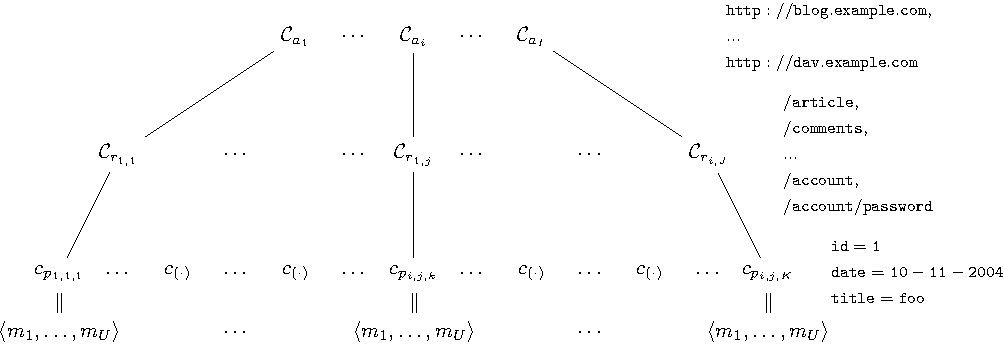
\includegraphics[angle=-90,width=.6\textwidth]{figures/web/profiles}
  \caption{Overview of web application model construction.}
  \label{fig:profiles}
\end{figure}

In addition to requests, the structure of user sessions can be taken
into account to model the normal states of a server-side
application. In this case, the anomaly detector does not consider
individual requests independently, but models their sequence. This
model captures the legitimate order of invocation of the resources,
according to the application logic. An example is when a user is
required to invoke an authentication resource (e.g.,
\texttt{/user/auth}) before requesting a private page (e.g.,
\texttt{/user/profile}). In~\citep{kruegel:jcn2005:webanomaly}, a
session $S$ is defined as a sequence of resources in $R$. For
instance, given $R = \{r_{1}, r_{2}, \dots, r_{10}\}$, a sample
session is $S = \langle r_{3}, r_{1}, r_{2}, r_{10}, r_{2}\rangle$.

Some systems also model \ac{HTTP}\index{HTTP} responses that are
returned by the server. For example,
in~\citep{kruegel:jcn2005:webanomaly}, a model $\mdoc$ is presented
that takes into account the structure of documents (e.g.,
\ac{HTML}\index{HTML}, \ac{XML}\index{XML}, and \ac{JSON}\index{JSON})
in terms of partial trees that include security-relevant nodes (e.g.,
\texttt{<script />} nodes, nodes containing \ac{DOM}\index{DOM} event
handlers, and nodes that contain sensitive data such as credit card
numbers). These trees are iteratively merged as new documents are
observed, creating a superset of the allowed document structure and
the positions within the tree where client-side code or sensitive data
may appear. A similar approach is adopted
in~\citep{masibty}.

\begin{note}[Web Application Behavior]
  The concept of \emph{web application behavior}, used in the
  following, is a particular case of the system behavior as defined by
  Definition~\ref{def:system-behavior}. Depending on the accuracy of
  each model, the behavior of a web application reflects the
  characteristics and functionalities that the application offers and,
  as a consequence, the content of the inputs (i.e., the requests)
  that it process and the outputs (i.e., the responses) that it
  produces. Thus, unless differently stated, we use the same term to
  indicate both the ideas.
\end{note}

After training, the system is switched to \emph{detection mode}, which
is performed online. The models trained in the previous phase are
queried to determine whether or not the new parameters observed are
anomalous. Without going into the details of a particular
implementation, each parameter is compared to all the applicable
models and an aggregated anomaly score between 0 and 1 is calculated
by composing the values returned by the various models. If the anomaly
score is above a certain threshold, an alert is generated. For
example, in~\citep{kruegel:acsac2003:bayesian}, the anomaly score
represents the probability that a parameter value is anomalous and it
is calculated using a Bayesian network that encodes the probability
that a parameter value is actually normal or anomalous given the
scores returned by the individual models.

\subsection{A Comprehensive Detection System to Mitigate Web-based
  Attacks}
\label{web:intro:masibty}
The approach described in~\citep{kruegel:jcn2005:webanomaly} are
further exploited in a recent work, \citep{masibty}, which we
partially contributed to. In particular, we defined a web application
anomaly detector that is able to detect a real-world threats against
the clients (e.g., malicious \textsf{JavaScript}\index{JavaScript} code, trying to
exploit browser vulnerabilities), the application (e.g., cross-site
scripting, permanent content injection), and the database layer (e.g.,
SQL injection). A prototype of the system, called \masibty, has been
evaluated on a set of real-world attacks against publicly available
applications, using both simple and mutated versions of exploits, in
order to assess the resilience to evasion. \masibty has the following
key characteristics:

\begin{itemize}
\item its models are designed with the explicit goal of not requiring
  an attack-free dataset for training, which is an unrealistic
  requirement in real-world applications. Even if in
  \citep{10.1109/SP.2008.11} techniques are suggested to filter
  outliers (i.e., attacks) from the training data, in absence of a
  ground truth there can be no guarantee that the dataset will be
  effectively free of attacks. Using such techniques before training
  \masibty would surely improve its detection capabilities.

\item As depicted in Figure~\ref{fig:masibty-architecture}, \masibty
  intercepts and process both HTTP requests (i.e., \emph{PAnomaly})
  and responses (i.e., \emph{XSS\-Anomaly}) and protects against both
  server-side and client-side attacks, an extremely important feature
  in the upcoming ``Web 2.0'' era of highly interactive websites based
  mainly on user contributed content. In particular, we devised two
  novel anomaly detection models --- referred to as ``engines'' ---
  based on the representation of the responses as trees.

\item \masibty incorporates an optional data protection component,
  i.e., \emph{QueryAnomaly} that extracts and parses the SQL queries
  sent to the database server. This component is part of the analysis
  of HTTP requests, and thus is not merely a reverse proxy to the
  database. In fact, it allows to bind the requests to the SQL queries
  that they generate, directly or indirectly. Hence, queries can be
  modeled although are not explicitly passed as a parameter of the
  HTTP requests.
\end{itemize}

\begin{figure}[p]
  \begin{center}
    \hspace*{2.5cm}
    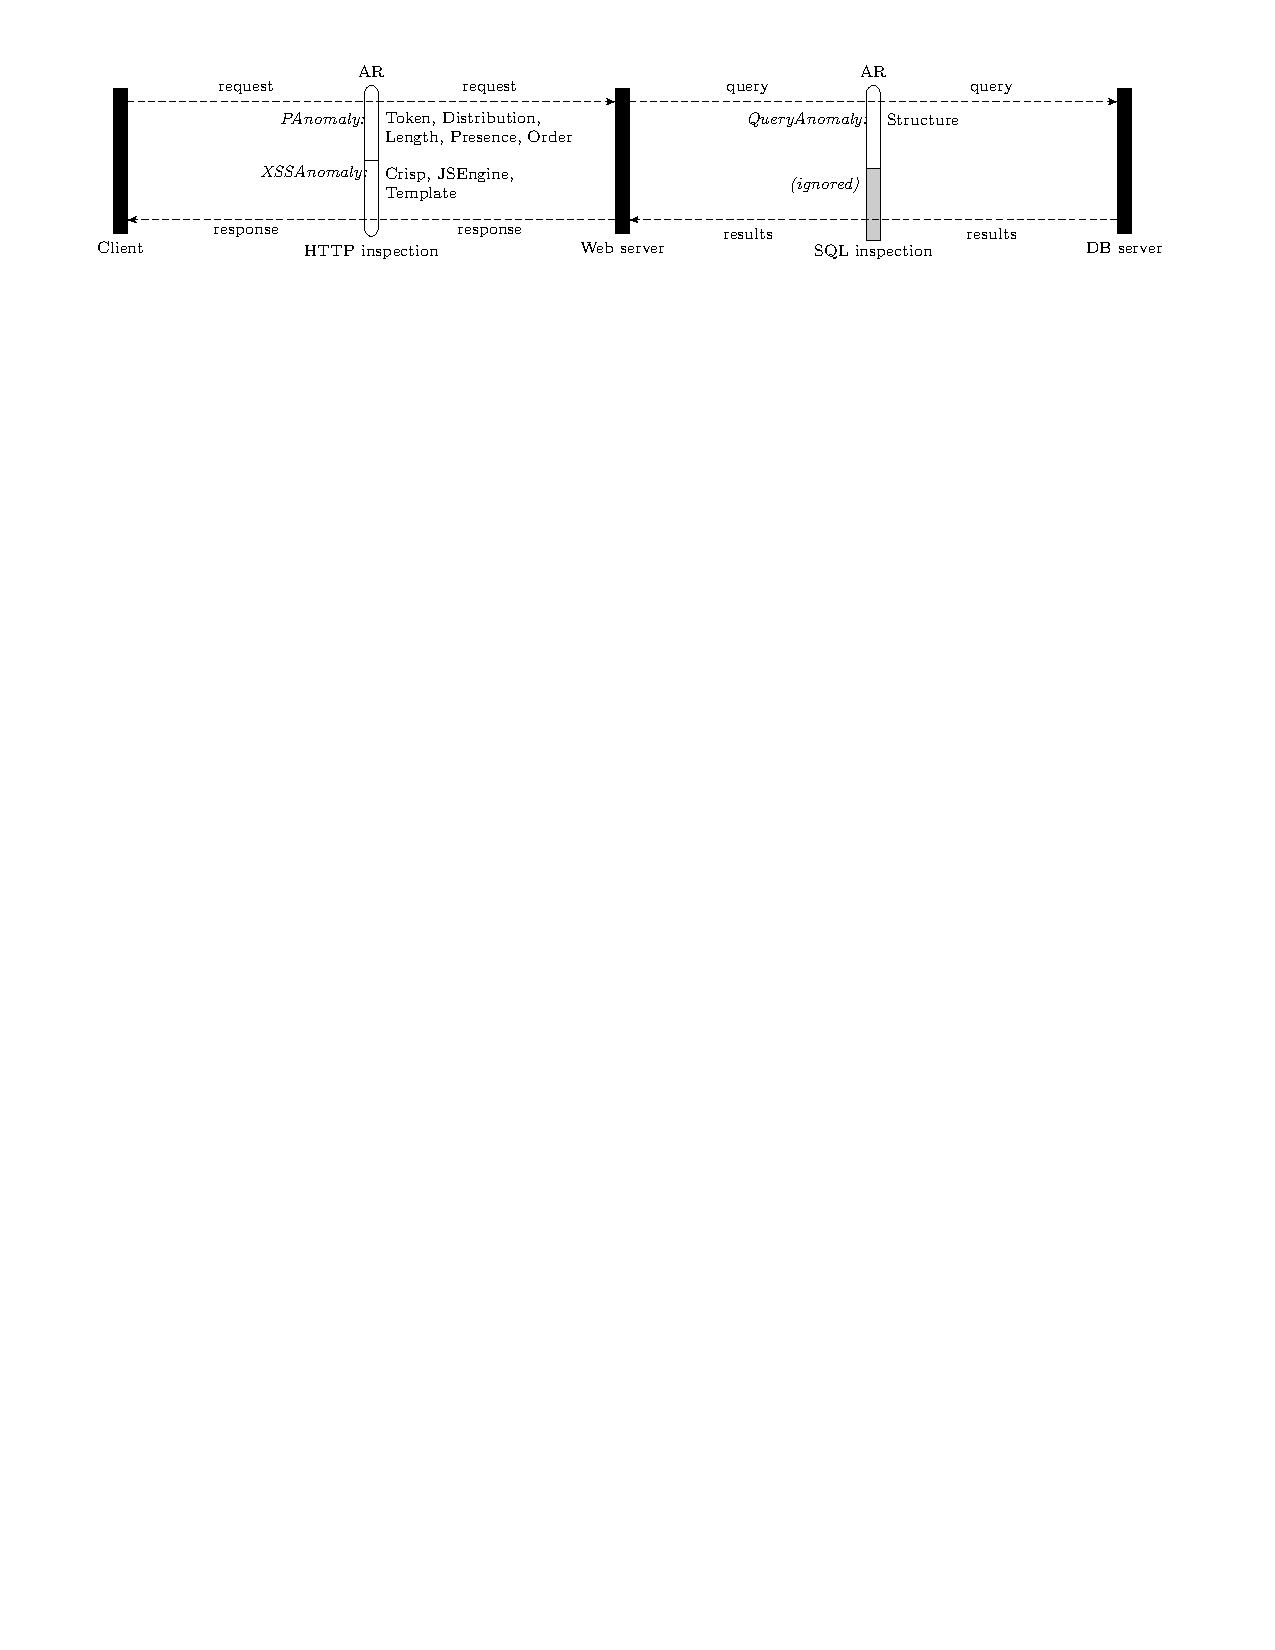
\includegraphics[angle=90,scale=.8]{figures/web/masibty/masibty-architecture}
  \end{center}

  \vspace*{-1cm}
  \caption{The logical structure of \masibty.}
  \label{fig:masibty-architecture}
\end{figure}

\subsection{Evaluation Data}
\label{web:intro:eval}
The experiments in Section~\ref{web:longtail} and \ref{web:conceptdrift} were conducted using a dataset drawn from real-world web applications deployed on both academic and industry web servers.  Examples of representative applications include payroll processors, client management, and online commerce sites.  For each application, the full content of each \ac{HTTP}\index{HTTP} connection observed over a period of several months was recorded.  The resulting flows were then filtered using the most advanced signature-based detection system, \textsf{Snort}\footnote{Source and attack signatures available for download at \url{http://snort.org}.}, to remove known attacks.  In total, the dataset contains 823 distinct web applications, 36,392 unique resource paths, 16,671 unique parameters, and 58,734,624 \ac{HTTP}\index{HTTP} requests.

\begin{note}[Dataset privacy]
  To preserve the privacy, the dataset used has been given to the Computer Security Laboratory of UC Santa Barbara under strict contractual agreements that denies to disclose specific information identifying the web applications themselves.
\end{note}

Two sets of 100,000 and 1,000 attacks was introduced into the dataset used for the approach described in Section~\ref{web:longtail} and \ref{web:conceptdrift}, respectively. These attacks were real-world examples and variations upon \ac{XSS} (e.g., CVE-2009-0781), \ac{SQL} injections (e.g., CVE-2009-1224), and command execution exploits (e.g., CVE-2009-0258) that manifest themselves in request parameter values, which remain the most common attacks against web applications. Representative examples of these attacks include:

\begin{itemize}
\item malicious JavaScript\index{JavaScript} inclusion
\begin{lstlisting}[numbers=none]
  <script src="http://example.com/malware.js"></script>
\end{lstlisting}
\item bypassing login authentication
\begin{lstlisting}[numbers=none]
  ' OR 'x'='x'--
\end{lstlisting}
\item command injection
\begin{lstlisting}[numbers=none]
  cat /etc/passwd | mail attacker@gmail.com \#
\end{lstlisting}

\end{itemize}

More precisely, the \ac{XSS}\index{XSS} attacks are variations on those listed in \citep{xss_cheat_sheet}, the \ac{SQL}\index{SQL} injections were created similarly from \citep{sqli_cheat_sheet}, and the command execution exploits were variations of common command injections against the \textsf{Linux} and \textsf{Windows} platforms.

\section{Training With Scarce Data}
\label{web:longtail}
In this section, we describe our contributions \citep{2009_robertson_maggi_kruegel_vigna} to cope with the difficulty of obtaining sufficient \emph{amounts} of training data. As we explained in Section~\ref{detection:ad:host} and \ref{detection:evaluation:issues}, this limitation has heretofore not been well studied. We developed this technique to work with \webanomaly and, in general, to any learning-based anomaly detection system against web attacks. In fact, the problem described in the following is significantly evident in the case of web applications. However, it can be easily applied to other anomaly-based system, as long as they rely on behavioral models and learning techniques such as those described in Section~\ref{host:syscall}.

The issue that motivates this work is that the number of web application component invocations is non-uniformly distributed. In fact, we noticed that relatively few components are dominant in the traffic and the remainder components are accessed relatively infrequently. Therefore, for those components, it is difficult to gather enough training data to accurately model their normal behavior.  In statistics, the infrequently accessed population is known as the ``long tail''. Note that, however, this does not necessarily imply a power law distribution. Clearly, components that are infrequently accessed lead to undertrained models (i.e., models that do not capture the normal behavior accurately). Consequently, models are subject to overfitting\index{overfitting} due to lack of data, resulting in increases in the \ac{FPR}.

In particular, in this section, we describe our joint work with UC Santa Barbara in which we propose to mitigate this problem by exploiting natural similarities among all web applications. In particular, we show that the values of the parameters extracted from \ac{HTTP}\index{HTTP} requests can generally be categorized according to their type, such as an integer, date, or string.  Indeed, our experiments demonstrate that parameters of similar type induce similar models of normal behavior.  This result is then exploited to supplement a local scarcity of training data for a given web application component with similar data from other web applications.

This section is structured as follows. In Section~\ref{web:longtail:motivation} the problem of the non-uniform distribution to the different components of a web application is discussed. In addition, we provide evidence that it occurs in the real world. In Section~\ref{web:longtail:design} approach to address the problem of model profile undertraining\index{undertraining} by using the notion of \emph{global profiles} that exploit similarities between web application parameters of similar type. In Section~\ref{web:longtail:eval} the application of global profiles is evaluated on a large dataset of real-world traffic from many web applications, and demonstrate that utilizing global profiles allows anomaly detectors to accurately model web application components that would otherwise be associated with undertrained models.

\subsection{Non-uniformly distributed training data}
\label{web:longtail:motivation}
To describe the undertraining\index{undertraining} problem, in this section we refer to the aforementioned, generic architecture of a web-based anomaly detector. To address the problem of undertraining\index{undertraining}, we leverage the set of models described in the Example~\ref{ex:web-models}.

Because anomaly detection systems dynamically learn specifications of
normal behavior from training data, it is clear that the quality of
the detection results critically relies upon the quality of the
training data. For example, as mentioned in
Section~\ref{detection:evaluation:issues}, a training dataset should
be attack-free and should accurately represent the normal behavior of
the modeled features. To our knowledge, the difficulty of obtaining
sufficient amounts of training data to accurately model web
applications is less well-known. In a sense, this issue is similar to
those addressed by statistical analysis methods with missing
data~\citep{little1987statistical}. Although a training procedure would
benefit from such mechanisms, they require a complete redesign of the
training algorithm specific to each model. Instead, a non-obtrusive
approach that can improve an existing system without modifying the
undertrained models is more desirable.  Typically, anomaly-based
detectors cannot assume the presence of a testing environment that can
be leveraged to generate realistic training data that exercises the
web application in a safe, attack-free environment. Instead, an
anomaly detection system is typically deployed in front of live web
applications with no \emph{a priori} knowledge of the applications'
components and their behavior.

In particular, in the case of low-traffic web applications, problems
arise if the rate of client requests is inadequate to allow models to
train in a timely manner. Even in the case of high-traffic web
applications, however, a large subset of resource paths might fail to
receive enough requests to adequately train the associated models.
This phenomenon is a direct consequence of the fact that resource path
invocations issued by web clients often follow a non-uniform
distribution.  To illustrate this point, Figure~\ref{fig:long_tail}
plots the normalized cumulative distribution function of web client
resource path invocations for a variety of real-world, high-traffic
web applications (details on the source of this data are provided in
Section~\ref{web:longtail:eval}). Although several applications have
an approximately uniform client access distribution, a clear majority
exhibits highly skewed distributions.  Indeed, in many cases, a large
percentage of resource paths receive a comparatively minuscule number
of requests. Thus, returning to the example mentioned in
Section~\ref{web:intro:ad}, assuming an overall request volume of
500,000 requests per day, the resource path set would result in the
client access distribution detailed in
Table~\ref{tab:client-access-distribution}.

\begin{table}[t]
  \centering
  \begin{tabular}{rl}
    \toprule
    \textsc{Resource Path} & \textsc{Requests}\\
    \midrule

    \texttt{/article} & 95.0\% \\
    \texttt{/comments} & 3.0\% \\
    \texttt{/comments/edit} & 1.8\% \\
    \texttt{/account} & 0.2\% \\
    \texttt{/account/password} & 0.02\%\\
    \bottomrule
  \end{tabular}

  \caption{Client access distribution on a real-world web application (based on 500,000 requests per day).}
  \label{tab:client-access-distribution}
\end{table}

Profiles for parameters to resource paths such as \texttt{/article} will receive ample training data, while profiles associated with account components will be undertrained. The impact of the problem is also magnified by the fact that components of a web application that are infrequently exercised are also likely to contain a disproportionately large portion of security vulnerabilities.  This could be a consequence of the reduced amount of testing that developers invariably perform on less prominent components of a web application, resulting in a higher rate of software flaws.  In addition, the relatively low request rate from users of the web application results in a reduced exposure rate for these flaws.  Finally, when flaws are exposed and reported, correcting the flaws may be given a lower priority than those in higher traffic components of a web application.

\begin{figure}[t]
  \centering
  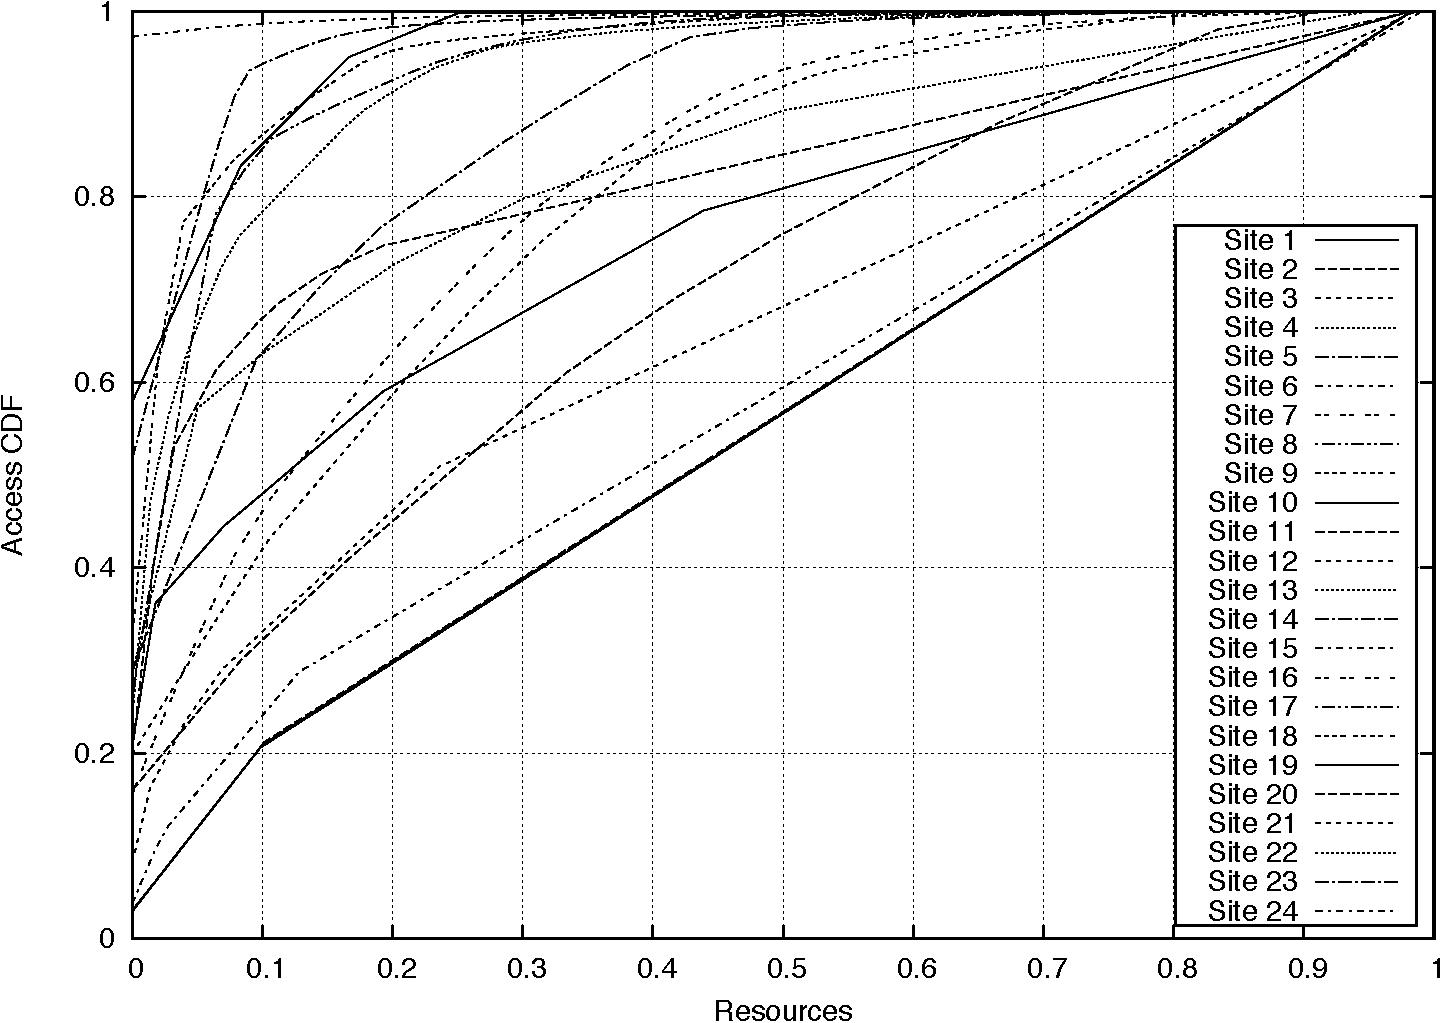
\includegraphics[width=.85\textwidth]{figures/web/longtail/fig_long_tail}
  \caption{Web client resource path invocation distributions from a
    selection of real-world web applications.}
  \label{fig:long_tail}
\end{figure}

\subsection{Exploiting global knowledge}
\label{web:longtail:design}
The approach described in this section is based on a key observation: parameters associated with the invocation of components belonging to different web applications often exhibit a marked similarity to each other. For instance, many web applications take an integer value as a unique identifier for a class of objects such as a blog article or comment, as in the case of the \texttt{id} parameter.  Similarly, applications also accept date ranges similar to the \texttt{date} parameter as identifiers or as constraints upon a search request.  Similarly, as in the case of the \texttt{title} parameter, web applications often expect a short phrase of text as an input, or perhaps a longer block of text in the form of a comment body. In some sense, each of these groupings of similar parameters can be considered as distinct \emph{parameter types}, though this need not necessarily correspond to the concept of types as understood in the programming languages context.

Our approach is based in the following assumption. Parameters of the
same type tend to induce model compositions that are similar to each
other in many respects. Consequently, if the lack of training data for
a subset of the components of a web application prevents an anomaly
detection system from constructing accurate profiles for the
parameters of those components, we claim that it is possible to
substitute, with an acceptably low decrease in the \ac{DR}, profiles
for similar parameters of the same type that were learned when enough
training data was available to construct accurate profiles. It must be
underlined that the substitution operates at the granularity of
\emph{parameters} rather than \emph{requests} (which may contain more
than one parameter). This increases the likelihood of finding
applicable profile similarities, and allows for the substitution of
models taken from radically different components.  However, although
the experiments on real-world data, described in
Section~\ref{web:longtail:eval}, confirm that the aforementioned
insight is realistic, our hypothesis might not hold in some very
specific settings. Thus, to minimize the risks brought by migrating
global knowledge across different deployments, we interpreted this
result only as an insight and developed a robust criterion able to
find similar profiles independently from the actual types of the
modeled parameters.

\begin{figure*}
  \centering
  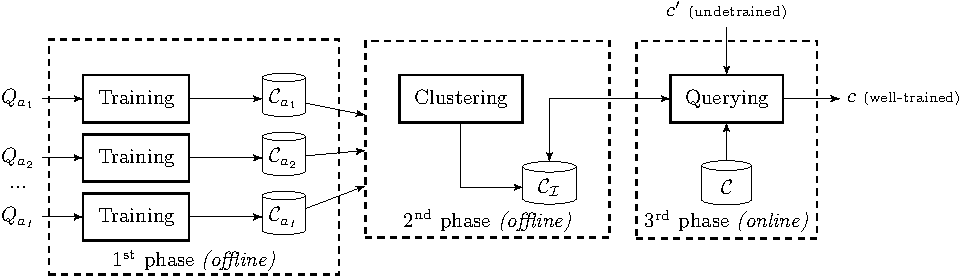
\includegraphics[width=\textwidth]{figures/web/longtail/overview}

  \caption{Overall procedure. Profiles, both undertrained and well-trained, are collected from a set of web applications. These profiles are processed offline to generate the global knowledge base $\kb$ and index $\kb^I$. $\kb$ can then be queried to find similar global profiles.}
  \label{fig:overview}
  
  \vspace*{-.4cm}
\end{figure*}

As schematized in Figure~\ref{fig:overview} our approach is composed of three phases.

\begin{description}
\item [First phase] (offline) Enhancement of the training procedure originally implemented in~\citep{kruegel:jcn2005:webanomaly}.

\item[Second phase] (offline) It is divided into three sub-steps.

  \begin{enumerate}
  \item A \emph{global knowledge base} of profiles $\kb=\bigcup_{a_i}\kb_{a_i}$ is constructed, where $\kb_{a_i}$ are knowledge bases containing only well-trained, stable profiles from anomaly detection systems previously deployed on a set of web applications $\bigcup_{i}a_i$.
  \item A knowledge base $\kb^I=\bigcup_{a_i}\kb_{a_i}^I$ of undertrained profiles is then constructed as an \emph{index} into $\kb$, where $\kb_{a_i}^I$ is a knowledge base of undertrained profiles from the web application $a_i$.
  \item Finally, a \emph{mapping} $f:\left\{\kb^I\right\}\times\kb_{a_i}\mapsto\kb$ is defined.
  \end{enumerate}

\item[Third phase] (online) For any new web application where insufficient training data is available for a component's parameter, the anomaly detector first extracts the undertrained profile $c'$ from the local knowledge base $\kb_{a_i}$.  Then, the global knowledge base $\kb$ is queried to find a similar, previously constructed profile $f\left(\kb_I,c'\right)=c\in\kb$.  The well-trained profile $c$ is then substituted for the undertrained profile $c'$ in the detection process.
\end{description}

The following sections detail how $\kb_I$ and $\kb$ are constructed, and how $f$ maps elements in $\kb_I$ and $\kb_{a_i}$ to elements in $\kb$.

\subsubsection{First Phase: Enhanced Training}
\label{web:longtail:design:enhanced-training}
A significant refinement of the individual models described in~\citep{kruegel:jcn2005:webanomaly} is the criterion used to determine the length of the training phase.  An obvious choice is to fix a constant training length, e.g., a thousand requests.  Unfortunately, an appropriate training length is dependent upon the complexity of modeling a given set of features.  Therefore, we have developed an automated method that leverages two stop criteria, \emph{model stability} and \emph{model confidence}, to determine when a model has observed enough training samples to accurately approximate the normal behavior of a parameter.

\paragraph{Model Stability}
\label{web:longtail:design:enhanced-training:stability}
As new training samples are observed early in the training phase, the
state of a model typically exhibits frequent and significant change as
its approximation of the normal behavior of a parameter is updated.
Informally, in an information-theoretic sense, the average information
gain of new training samples is high.  As a model's state converges to
a more precise approximation of normal behavior, however, its state
exhibits infrequent and incremental changes.  In other words, the
information gain of new training samples approaches zero, and the
model stabilizes. Note that, we refer to the information gain as an
informal and intuitive concept to explain the rationale behind the
development of a sound model stability criterion. By no means we claim
that our procedure relies on the actual information gain to calculate
when a model converges to stability.

Each model self-assesses its stability during the training phase by maintaining a history of snapshots of its internal state.  At regular intervals, a model checks if the sequence of deltas between each successive historical state is monotonically decreasing and whether the degree of change drops below a certain threshold.  If both conditions are satisfied, then the model considers itself stable.  Let $\kappa_{\text{stable}}^{\left(u\right)}$ denote the number of training samples required for a model to achieve stability.  A profile is considered stable when all of its constituent models are stable.

\begin{definition}[Profile stability]
   Let $\kappa_{\text{stable}}$ be the number of training samples required for a single model to achieve stability. The \emph{aggregated stability} measure is defined as:

   \begin{equation}
     \kappa_{\text{stable}}=\max_{u\in
       U}\kappa_{\text{stable}}^{\left(u\right)}.
   \end{equation}
\end{definition}

The notion of model stability is also leveraged in the third phase, as detailed in Section~\ref{web:longtail:design:global}.

\begin{note}
  Instead of describing the internal stop criterion specific to each
  model, if any, we developed a model-agnostic minimization algorithm
  detailed in Section~\ref{web:longtail:design:mapping} (and evaluated
  in Section~\ref{web:longtail:eval:robustness}) that allows one to
  trade off detection accuracy against the number of training samples
  available.
\end{note}

\paragraph{Model Confidence}
\label{web:longtail:design:enhanced-training:confidence}
A related notion to model stability is that of \emph{model confidence}.  Recall that the goal of a model is to learn an abstraction of the normal behavior of a feature from the training data.  There exists a well-known tension in the learning process between accurately fitting the model to the data and generalizing to data that has not been observed in the training set.  Therefore, in addition to detecting whether a model has observed enough training samples to accurately model a feature, each model incorporates a self-confidence measure $z^{\left(u\right)}$ that represents whether the model has generalized so much as to lose all predictive power.

For example, the confidence of a token model should be directly related to the probability that a token set is present.

\begin{definition}[Token model confidence]
  The \emph{token model confidence} is defined as:

\begin{equation}
  z^{\left(\text{tok}\right)}=\tau=\frac{1}{2}+\frac{n_c-n_d}{4n\left(n-1\right)},
\end{equation}

where $n_c$ and $n_d$ are the number of concordant and discordant pairs, respectively, between the unique number of observed samples and the total number of samples observed at each training step, and $n$ is the total number of training samples.
\end{definition}

Note that, $z_{\mtok}$ is an adaptation of the $\tau$ coefficient~\citep{kendalltau}.

For the integer and length models, the generality of a particular model can be related to the statistical dispersion of the training set.

\begin{definition}[Integer model confidence]
  Given the observed standard deviation $\sigma$, minimum observed value $u$, and maximum observed value $v$, the \emph{confidence of an integer or length model} is defined as:

\begin{equation}
  z^{\left(\left\{\text{int,len}\right\}\right)}=
  \begin{cases}
    1-\frac{\sigma}{v-u} &\text{if } v-u>0 \\
    1 &\text{otherwise}
  \end{cases}.
\end{equation}
\end{definition}

The confidence of a character distribution model is determined by the variance of observed \acp{ICD}\index{ICD}.  Therefore, the confidence of this model is given by a similar construction as the previous one, except that instead of operating over observed values, the measure operates over observed variances.

\begin{definition}[Char. distr. model confidence]
  Given the standard deviation of observed variances $\sigma$, the minimum observed variance $u$, and the maximum observed variance $v$, the \emph{confidence of a character distribution model} is:

\begin{equation}
  z^{\left(\text{char}\right)}=
  \begin{cases}
    1-\frac{\sigma}{v-u} &\text{if } v-u>0 \\
    1 &\text{otherwise}
  \end{cases}.
\end{equation}
\end{definition}

Finally, the \ac{HMM}\index{HMM} induced by the structure model can be directly analyzed for generality.  We perform a rough estimate of this by computing the mean probability for any symbol from the learned alphabet to be emitted at any state.

\begin{definition}[Struct. model confidence]
  Given a structural model, i.e. an \ac{HMM}, specified by the tuple $\langle\mathbb{S},\mathbb{O},M_{\mathbb{S}\times\mathbb{S}}, P\left(\mathbb{S},\mathbb{O}\right),P\left(\mathbb{S}\right)\rangle$, where $\mathbb{S}$ is the set of states, $\mathbb{O}$ is the set of emissions, $M_{\mathbb{S}\times\mathbb{S}}$ is the state transition probability matrix, $P\left(\mathbb{S},\mathbb{O}\right)$ is the emission probability distribution over the set of states, and $P\left(\mathbb{S}\right)$ is the initial probability assignment, \emph{the structural model confidence}:

\begin{equation}
  z^{\left(\text{struct}\right)}=1-
  \frac{1}{\left|\mathbb{S}\right|\left|\mathbb{O}\right|}
  \sum_{i=1}^{\left|\mathbb{S}\right|}
  \sum_{j=1}^{\left|\mathbb{O}\right|}P\left(s_i,o_j\right).
\end{equation}
\end{definition}

At the end of this phase, for each web application $a_{i}$, the profiles are stored in the corresponding knowledge base $\kb_{a_{i}}$ and are ready to be processed by the next phase.

\subsubsection{Second Phase: Building a global knowledge base}
\label{web:longtail:design:global}
This phase is divided into the three sub-steps described in the following.

\paragraph{Well-trained profiles}
The construction of $\kb$ begins by merging a collection of knowledge bases $\left\{\kb_{a_1},\kb_{a_2},\ldots,\kb_{a_n}\right\}$ that have previously been built by a web application anomaly detector over a set of web applications $\bigcup_{i}a_i$.  The profiles in $\kb$ are then clustered in order to group profiles that are semantically similar to each other.  Profile clustering is performed in order to time-optimize query execution when indexing into $\kb$, as well as to validate the notion of parameter types.  In this work, an agglomerative hierarchical clustering algorithm using group average linkage was applied, although the clustering stage is, in principle, agnostic as to the specific algorithm.  For an in-depth discussion of clustering algorithms and techniques, we refer the reader to~\citep{clustering:survey}.

Central to any clustering algorithm is the distance function, which defines how distances between the objects to be clustered are calculated.  A suitable distance function must reflect the semantics of the objects under consideration, and should satisfy two conditions:

\begin{itemize}
\item the overall similarity (i.e., inverse of the distance) between elements within the same cluster is maximized, and
\item the similarity between elements within different clusters is minimized.
\end{itemize}

We define the distance between two profiles to be the sum of the distances between the models comprising each profile. More formally.

\begin{definition}[Profile distance]
  The \emph{distance between two profiles} $c_i$ and $c_j$ is defined as:

  \begin{equation}
    d\left(c_i,c_j\right)=\frac{1}{\left|c_i\bigcap c_j\right|}
    \sum_{m_i^{\left(u\right)},m_j^{\left(u\right)}\in c_i\bigcap c_j}
    \delta_u\left(m_i^{\left(u\right)},m_j^{\left(u\right)}\right),
    \label{eq:dist}
  \end{equation}
  
  where $\delta_u:\mathcal{M}_u\times\mathcal{M}_u\mapsto\left[0,1\right]$ is the distance function defined between models of type $u\in U=\left\{\text{tok}, \text{int}, \text{len}, \text{char}, \text{struct}\right\}$.
\end{definition}

The token model $\mtok$ is represented as a set of unique tokens observed during the training phase. Therefore, two token models $\mtok_i$ and $\mtok_j$ are considered similar if they contain similar sets of tokens.  More formally.

\begin{definition}[Token models distance]
  The \emph{distance function for token models} is defined as the Jaccard\index{Jaccard} distance~\citep{clustering:distance_metrics_survey}:

\begin{equation}
  \delta_{\text{tok}}\left(\mtok_i,\mtok_j\right)=
  1-\frac{\left|\mtok_i\bigcap\mtok_j\right|}{\left|\mtok_i\bigcup\mtok_j\right|}.
\end{equation}
\end{definition}

The integer model $\mint$ is parametrized by the sample mean $\mu$ and variance $\sigma$ of observed integers.  Two integer models $\mint_i$ and $\mint_j$ are similar if these parameters are also similar.

\begin{definition}[Integer models distance]
  The \emph{distance function for integer models} is defined as:

  \begin{equation}
    \delta_{\text{int}}\left(\mint_i,\mint_j\right)=
    \frac{\left\|\frac{\sigma_i^2}{\mu_i^2}-\frac{\sigma_j^2}{\mu_j^2}\right\|}
    {\frac{\sigma_i^2}{\mu_i^2}+\frac{\sigma_j^2}{\mu_j^2}}.
  \end{equation}
\end{definition}

\begin{note}[Length models distance]
  As the string length model is internally identical to the integer model, its distance function $\delta_{\text{len}}$ is defined similarly.
\end{note}

Recall that the character distribution model $\mchar$ learns the frequencies of individual characters comprising strings observed during the training phase.  These frequencies are then ranked and coalesced into a $n$ bins to create an \ac{ICD}\index{ICD}.  Two character distribution models $\mchar_i$ and $\mchar_j$ are considered similar if each model's \acp{ICD}\index{ICD} are similar. More formally.

\begin{definition}[Char. distr. models distance]
  The \emph{character distribution models distance} is defined as:
\begin{equation}
  \delta_{\text{char}}\left(\mchar_i,\mchar_j\right)=
  \sum_{l=0}^{n}\frac{\left\|b_i\left(l\right)-b_j\left(l\right)\right\|}
  {\max_{k=i,j}b_k\left(l\right)},
\end{equation}

where $b_i\left(k\right)$ is the value of bin $k$ for $\mchar_i$.
\end{definition}

The structural model $\mstruct$ builds an \ac{HMM}\index{HMM} by observing a sequence of character strings.  The resulting \ac{HMM}\index{HMM} encodes a probabilistic grammar that can produce a superset of the strings observed during the training phase.  The \ac{HMM}\index{HMM} is specified by the tuple $\langle\mathbb{S},\mathbb{O},M_{\mathbb{S}\times\mathbb{S}}, P\left(\mathbb{S},\mathbb{O}\right),P\left(\mathbb{S}\right)\rangle$.  Several distance metrics have been proposed to evaluate the similarity between \acp{HMM}\index{HMM}~\citep{hmm:metrics:1, hmm:metrics:2, hmm:metrics:3, hmm:metrics:4}.  Their time complexity, however, is non-negligible.  Therefore, we adopt a less precise, but considerably more efficient, distance metric between two structural models $\mstruct_i$ and $\mstruct_j$.

\begin{definition}[Struct. models distance]
  The \emph{structural models distance} is defined as the Jaccard\index{Jaccard} distance between their respective emission sets:

\begin{equation}
  \delta_{\text{struct}}\left(\mstruct_i,\mstruct_j\right)=
  1-\frac{\left|\mathbb{O}_i\bigcap\mathbb{O}_j\right|}
  {\left|\mathbb{O}_i\bigcup\mathbb{O}_j\right|}.
\end{equation}
\end{definition}

\paragraph{Undertrained profiles}
Once the global knowledge base $\kb$ has been built, the next step is to construct a knowledge base of undertrained models $\kb^I$.  This knowledge base is composed of profiles that have been deliberately undertrained on $\kappa\ll\kappa_{\text{stable}}$ for each of the web applications $a_i$.  Because each member of $\kb^I$ uniquely corresponds to a member in $\kb$ and undertrained profiles are built for each well-trained profile in $\kb$, a bijective mapping $f':\kb^I\mapsto\kb$ exists between $\kb^I$ and $\kb$.  Therefore, when a web application parameter is identified as likely to be undertrained, the corresponding undertrained profile $c'$ can be compared to a similar undertrained profile in $\kb^I$, which is then used to select a corresponding stable profile from $\kb$. This operation requires the knowledge base $\kb^{I}$ to be indexed. The construction of the indices relies on the notion of model stability, described in Section~\ref{web:longtail:design:enhanced-training:stability}.

\begin{figure}[t]
  \centering
  \begin{tikzpicture}[el/.style={circle,fill=black!75,inner sep=1pt,label={above right:#1}},every label/.style = {font=\footnotesize},every node/.style={font=\footnotesize},ci/.style={shape=rectangle,thin,draw,inner sep=2pt}]

    \foreach \p in {1, 2, ..., 7}
       \foreach \k in {1, 2, ..., 8}
         \node [el] at ($ (5.5,0) + .8*(\k,\p)$) (d_\k_\p) {};

     \foreach \p/\k in {1/1, 2/2, 3/4, 4/8, 5/16, 6/32, 7/64}
       \node at ($ (5.5,0) + .8*(0,\p)$) {$\kappa = \k$};

     \node [ci,fit=(d_1_1)] {}
      node [ci,fit=(d_2_1)] {}
      node [ci,fit=(d_4_1)] {}
      node [ci,fit=(d_5_1)] {}
      node [ci,fit=(d_6_1)] {}
      node [ci,fit=(d_7_1)] {};

      \node [ci,fit=(d_1_2) (d_2_2)] {}
       node [ci,inner sep=3.5pt,fit=(d_2_2) (d_3_2)] {}
       node [ci,fit=(d_4_2) (d_5_2)] {}
       node [ci,fit=(d_7_2) (d_8_2)] {};

     \node [ci,fit=(d_2_3) (d_3_3) (d_4_3) (d_5_3)] {}
      node [ci,inner sep=3.5pt,fit=(d_5_3) (d_6_3) (d_7_3) (d_8_3)] {};

      \node [ci,fit=(d_1_4) (d_8_4)] {};

     \node [rotate=90] at (13,3.25) {Requests in $Q^{\left(p\right)}$};

  \end{tikzpicture}
  \caption{Partitioning of the training set $Q$ for various $\kappa$.}
  \label{fig:slicing}
\end{figure}

The undertrained profiles that comprise $\kb^I$ are constructed using
the following procedure.  Let
$Q^{\left(p\right)}=\{q_1^{\left(p\right)},q_2^{\left(p\right)},\ldots\}$
denote a sequence of client requests containing parameter $p$ for a
given web application.  Over this sequence of requests, profiles are
deliberately undertrained on randomly sampled $\kappa$-sequences.
Each of the resulting profiles is then added to the set $\kb^I$.
Figure~\ref{fig:slicing} depicts this procedure for various $\kappa$.
Note that the random sub-sampling is performed with the goal of
inducing undertraining\index{undertraining} to show that clustering is feasible and leads
to the desired grouping even -- and especially -- in the presence of
undertraining\index{undertraining}.

Recall that $\kappa_{\text{stable}}$ is the number of training samples required for a profile to achieve stability.  Then, a profile is considered undertrained when the number of training samples it has observed, $\kappa$, is significantly less than the number required to achieve stability.  Therefore, an undertrained knowledge base $\kb^I$ is a set of profiles that have observed $\kappa$ samples such that $\kappa\ll\kappa_{\text{stable}}$.

The selection of an appropriate value for $\kappa$ is central to both
the efficiency and the accuracy of this process.  Clearly, it is
desirable to minimize $\kappa$ in order to be able to index into $\kb$
as quickly as possible once a parameter has been identified to be
subject to undertraining\index{undertraining} at runtime.  On the other hand, setting
$\kappa$ too low is problematic, as Figure~\ref{fig:clustering}
indicates.  For low values of $\kappa$, profiles are distributed with
relatively high uniformity within $\kb^I$, such that clusters in
$\kb^I$ are significantly different than clusters of well-trained
profiles in $\kb$.  Therefore, slight differences in the state of the
individual models can cause profiles that are close in $\kb^I$ to map
to radically different profiles in $\kb$.  As
$\kappa\rightarrow\kappa_{\text{stable}}$, however, profiles tend to
form meaningful clusters, and tend to approximate those found in
$\kb$.  Therefore, as $\kappa$ increases, profiles that are close in
$\kb^I$ become close in $\kb$ under $f$ -- in other words, $f$ becomes
\emph{robust} with respect to model semantics.

\begin{figure}[p]
  \centering 
  \begin{tikzpicture}[el/.style={circle,fill=black!75,inner sep=1pt,label={above right:#1}},every label/.style = {font=\footnotesize},every node/.style={font=\footnotesize},ci/.style={shape=rectangle,thin,draw,inner sep=2pt}]

    \node [el,label={above right:$c_{p_{1,1}}$}] at (0, 0) (1_p_1) {};
    \node [el,label={above right:$c_{p_{2,1}}$}] at (0.5, 0.75) (1_p_2) {};
    \node [el,label={above right:$c_{p_{3,1}}$}] at (0, 1.5) (1_p_3) {} ;
    \node [el,label={above right:$c_{p_{4,1}}$}] at (-0.5, 0) (1_p_4) {};
    \node [el,label={above right:$c_{p_{5,1}}$}] at (1, 0.5) (1_p_5) {}; 

    \node [el,label={above right:$c_{p_{6,1}}$}] at (0, 1) (1_p_6) {};
    \node [el,label={above right:$c_{p_{7,1}}$}] at (0.5, 1.75) (1_p_7) {};

    \node [el,label={above right:$c_{p_{8,1}}$}] at (-1, 1) (1_p_8) {};
    \node [el,label={above right:$c_{p_{9,1}}$}] at (-1.5, 1.6) (1_p_9) {};
    \node [el,label={above right:$c_{p_{10,1}}$}] at (-1.25, 1.4) (1_p_10) {};

     \foreach \k/\name/\l in {3/2/2, 6/4/4, 8.5/K/\kappa}
       \foreach \i in {1, 2, ..., 10}
         \node [el,label={above right:$c_{p_{\i,\l}}$}] at ($ (1_p_\i) + (-1/\k*rand,\k) $) (\name_p_\i) {};
    
    \foreach \i in {1, 2, ..., 10}
         \node [el,label={above right:$c_{p_{\i}}$}] at ($ (K_p_\i) + (0,3) $) (s_p_\i) {};

     \foreach \k/\name in {1/1, 3/2, 6/4, 8.5/K}
       \foreach \i in {1, 2, ..., 10}
         \foreach \j in {1, 2, ..., 10}
           \fill [black,opacity=.45] ($ (\name_p_\i) + 0.8/\k*(rand,rand) $) circle (.7pt);

     \foreach \from/\to in {1/2, 2/4, 4/K}
       \foreach \i in {1, 2, ..., 10}
         \draw [opacity=.35] (\from_p_\i) -- (\to_p_\i);

    \node [el,inner sep=1.5pt,label={above right:$\mathbf{c}$}] at ($(K_p_8) - (.4, .4) $) (p) {};
    \node [circle,draw=black,inner sep=10pt,fill=black,opacity=.18] at ($ (p) $) (pn) {};
    \draw [-stealth] (p) to ($ (pn) - (10pt,10pt) $) {} node at ($ (p) - (.1,.25) $) {};
    \node [circle,draw=black,inner sep=15pt,fill=black,opacity=.15] at ($ (p) $) (pnn) {};
    \draw [-stealth] (p) to ($ (pn) - (22pt,0) $) {} node at ($ (p) - (.25,-.2) $) {};

    \draw [-stealth,dashed] (p) to [bend left=25] ($ (s_p_8) - (0.25,0)$) {};

     \node [draw = black!35, inner sep=5pt, thin, ellipse, fit = (1_p_1) (1_p_2) (1_p_3) (1_p_4) (1_p_5) (1_p_6) (1_p_7) (1_p_8) (1_p_9) (1_p_10)]{};

     \node [draw = black!35, inner sep=0pt, thin, ellipse, fit = (2_p_8) (2_p_9) (2_p_10)]{};
     \node [draw = black!35, inner sep=0pt, thin, ellipse, fit = (2_p_4)]{};
     \node [draw = black!35, inner sep=0pt, thin, ellipse, fit = (2_p_1) (2_p_2) (2_p_3) (2_p_5) (2_p_6) (2_p_7)]{};

     \node [draw = black!35, inner sep=0pt, thin, ellipse, fit = (4_p_8) (4_p_9) (4_p_10)]{};
     \node [draw = black!35, inner sep=0pt, thin, ellipse, fit = (4_p_1) (4_p_4) (4_p_5)]{};
     \node [draw = black!35, inner sep=0pt, thin, ellipse, fit = (4_p_2) (4_p_3) (4_p_6) (4_p_7)]{};

     \node [draw = black!35, inner sep=0pt, thin, ellipse, fit = (K_p_8) (K_p_9) (K_p_10)] {};
     \node [draw = black!35, inner sep=0pt, thin, ellipse, fit = (K_p_6) (K_p_5) (K_p_2)] {};
     \node [draw = black!35, inner sep=0pt, thin, ellipse, fit = (K_p_1) (K_p_4)] {};
     \node [draw = black!35, inner sep=0pt, thin, ellipse, fit = (K_p_3) (K_p_7)] {};

     \node [draw = black!35, inner sep=0pt, thin, ellipse, fit = (s_p_8) (s_p_9) (s_p_10)] {};
     \node [draw = black!35, inner sep=0pt, thin, ellipse, fit = (s_p_6) (s_p_5) (s_p_2)] {};
     \node [draw = black!35, inner sep=0pt, thin, ellipse, fit = (s_p_1) (s_p_4)] {};
     \node [draw = black!35, inner sep=0pt, thin, ellipse, fit = (s_p_3) (s_p_7)] {};

     \foreach \i/\k in {-1/0, 2.5/1, 5.5/2, 8.25/4, 11/\kappa_{min}, 14/{\kappa_{stable} \gg \kappa_{min}}}
       \draw [black!40] (-3, \i) to (3, \i) {}
         node [color=black,right] {$\kappa = \k$};

     \node at (-3, 0.75) {$\mathcal{C}_{1}^{I}$};
     \node at (-3, 4) {$\mathcal{C}_{2}^{I}$};
     \node at (-3, 6.75) {$\mathcal{C}_{4}^{I}$};
     \node at (-3, 9.5) {$\mathcal{C}_{\kappa_{min}}^{I}$};
     \node [rotate=90] at (11, 9.5) {Well-trained};
     \node at (10, 9.5) {$\mathcal{C}$};

     \node at ($ (K_p_7) + (1,1) $) {};
     
   \end{tikzpicture}

  \caption{Procedure for building global knowledge base indices.}
  \label{fig:clustering}
  \vspace*{-.4cm}
\end{figure}

\begin{note}[Robustness]
  Our use of the term ``robustness'' is related, but not necessarily equivalent, to the definition of robustness in statistics (i.e., the property of a model to perform well even in the presence of small changes in the underlying assumptions).
\end{note}

\paragraph{Mapping undertrained profiles to well-trained profiles}
\label{web:longtail:design:mapping}
A principled criterion is required for balancing quick indexing against a robust profile mapping.  Accordingly, we first construct a candidate knowledge base $\kb_{\kappa}^I$ for a given $\kappa$, as in the case of the global knowledge base construction.  Then, we define a \emph{robustness metric} as follows.  Let $H^I=\bigcup_{i}h_i^I$ be the set of clusters in $\kb^I$, and $H=\bigcup_{i}h_i$ be the set of clusters in $\kb$.  Let $g:H^I\mapsto\mathbb{N}$ be a mapping from an undertrained cluster to the maximum number of elements in that cluster that map to the same cluster in $\kb$.  The robustness metric $\rho:\left\{\kb^I\right\}\mapsto\left[0,1\right]$ is then defined as

\begin{equation}
  \rho\left(\kb^I\right)=\frac{1}{\left|\kb^I\right|}\sum_{i}g\left(h_i^I\right).
\end{equation}

With this metric, an appropriate value for $\kappa$ can now be chosen as

\begin{equation}
  \kappa_{\text{min}}=\min_{\kappa}\left(\rho\left(\kb_{\kappa}^I\right)\geq \rho_{\text{min}}\right),
\end{equation}

where $\rho_{\text{min}}$ is a minimum robustness threshold.

With the construction of a global knowledge base $\kb$ and an undertrained knowledge base $\kb^I$, online querying of $\kb$ can then be performed.

\subsubsection{Third Phase: Querying and Substitution}
Given an undertrained profile $c'$ from an anomaly detector deployed over a web application $a_i$, the mapping $f:\left\{\kb^I\right\}\times\kb_{a_i}\mapsto\kb$ is defined as follows.  A nearest\hyp{}neighbor match is performed between $c'$ and the previously constructed clusters $H^I$ from $\kb^I$ to discover the most similar cluster of undertrained profiles.  This is done to avoid a full scan of the entire knowledge base, which would be prohibitively expensive due to the cardinality of $\kb^I$.

Then, using the same distance metric defined in Equation~\eqref{eq:dist}, a nearest-neighbor match is performed between $c'$ and the members of $H^I$ to discover the most similar undertrained profile $c^I$.  Finally, the global, well-trained profile $f'\left(c^I\right)=c$ is substituted for $c'$ for the web application $a_i$.

To make explicit how global profiles can be used to address a scarcity
of training data, consider the example introduced in
Section~\ref{web:intro:ad}.  Since the resource path
\texttt{/account/password} has received only 100 requests (see
Table~\ref{tab:client-access-distribution}: \texttt{/account/password}
has received $0.02\%$ of 500,000 total requests), the profiles for
each of its parameters
$\left\{\mathtt{id},\mathtt{oldpw},\mathtt{newpw}\right\}$ are
undertrained, as determined by each profile's aggregate stability
measure.  In the absence of a global knowledge base, the anomaly
detector would provide no protection against attacks manifesting
themselves in the values passed to any of these parameters.

If, however, a global knowledge base and index are available, the situation is considerably improved.  Given $\kb$ and $\kb^I$, the anomaly detector can simply apply $f$ for each of the undertrained parameters to find a well-trained profile from the global knowledge base that accurately models a parameter with similar characteristics \emph{from another web application}.  Then, these profiles can be substituted for the undertrained profiles for each of $\left\{\mathtt{id},\mathtt{oldpw},\mathtt{newpw}\right\}$.  As will be demonstrated in the following section, the substitution of global profiles provides an acceptable detection accuracy for what would otherwise be an unprotected component (i.e., without a global profile 0\% of the attacks against that component would be detected).

\begin{note}[HTTP parameters ``semantics'']
  It is important to underline that the goal of this approach is not
  that of understanding the types of the fields nor their
  semantic. However, if the system administrator and the security
  officer had enough time and skills, the use of manual tools such as
  live debuggers or symbolic execution engines may help to infer the
  types of the fields and, once available, this information may be
  exploited as a lookup criterion. Unfortunately, this would be a
  human-intensive task, thus far from being automatic.

  Instead, our goal is to find groups of similar models, regardless of
  what this may imply in terms of types. According to our experiments,
  similar models tend to be associated to similar types. Thus, in
  principle, our method cannot be used to infer the parameters' types
  but can certainly give insights about parameters with similar
  features.
\end{note}

\subsection{Experimental Results}
\label{web:longtail:eval}
The goal of this evaluation is three-fold.  First, we investigate the
effects of profile clustering, and support the hypothesis of parameter
types by examining global knowledge base clusters.  Then, we discuss
how the quality of the mapping between undertrained profiles and
well-trained profiles improves as the training slice length $\kappa$
is increased.  Finally, we present results regarding the accuracy of a
web application anomaly detection system incorporating the application
of a global knowledge base to address training data scarcity.

\subsubsection{Profile clustering quality}
\label{web:longtail:eval:clustering}

\begin{figure}[p]
  \centering
  \subfloat[][$\kappa = 64$] {
    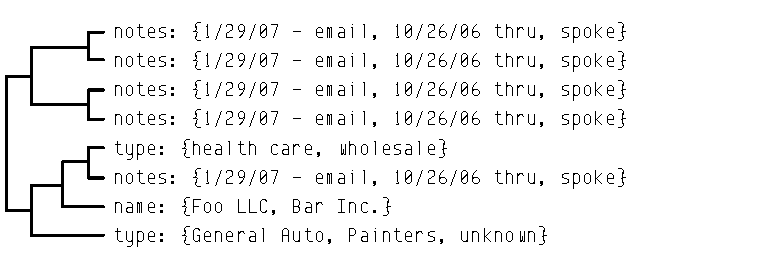
\includegraphics[scale=.5]{figures/web/longtail/undertrained-site-1-k-64-o}
    \label{subfig:undertrained-site-1-k-64}
  }\\
  \subfloat[][$\kappa_{stable} \simeq 10^{3}$] {
    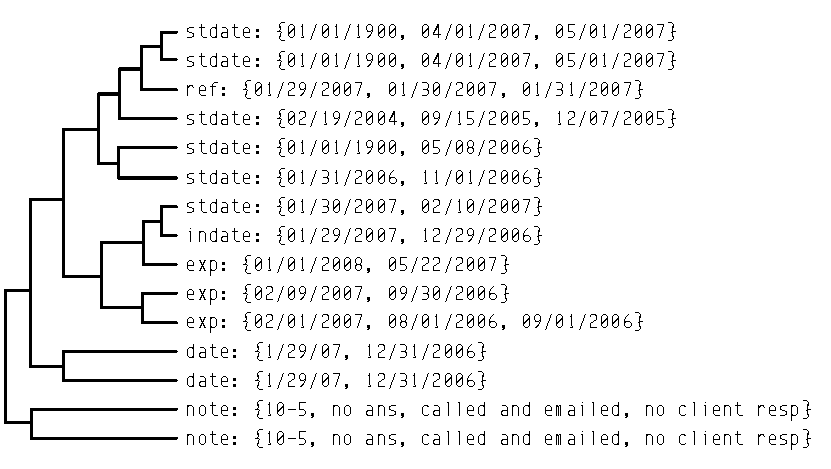
\includegraphics[scale=.5]{figures/web/longtail/undertrained-site-1-k-stable-o}
    \label{subfig:undertrained-site-1-k-stable}
  }\\
  \subfloat[][$\kappa = 8$]{
    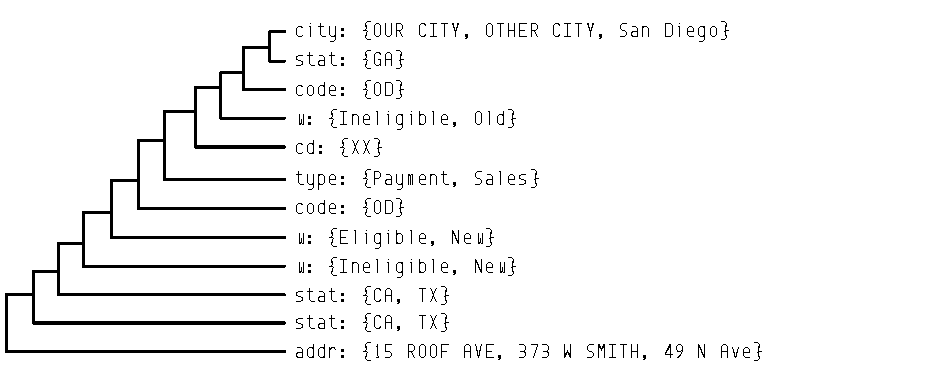
\includegraphics[scale=.5]{figures/web/longtail/undertrained-site-1-k-8-o}
    \label{subfig:undertrained-site-1-k-8}
  }\\
  \subfloat[][$\kappa = 32$]{
    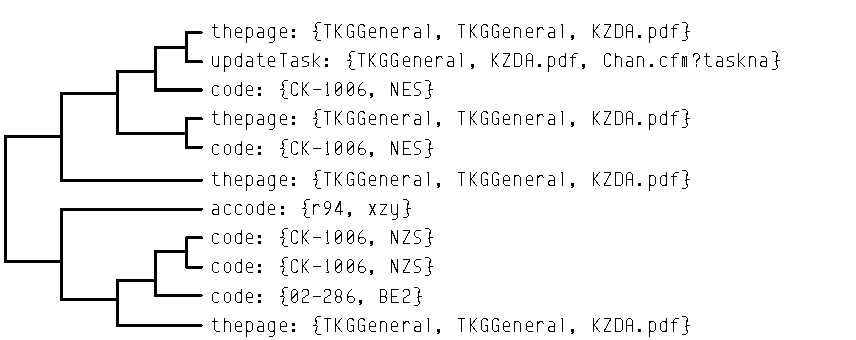
\includegraphics[scale=.5]{figures/web/longtail/undertrained-site-1-k-32-o}
    \label{subfig:undertrained-site-1-k-32}
  }\\
  \caption{Clustering of $\kb$, (a-b), and $\kb^I$, (c-d). Each leaf (a profile) is labeled with the parameter name and samples values observed during training. As $\kappa$ increases, profiles are clustered more accurately.}
  \label{fig:dendrograms}
  \vspace*{-.5cm}
\end{figure}

To evaluate the accuracy of the clustering phase, we first built a global knowledge base $\kb$ from a collection of well-trained profiles.  The profiles were trained on a subset of the data mentioned in Section~\ref{web:intro:eval}; this subset was composed of 603 web applications, 27,990 unique resource paths, 9,023 unique parameters, and 3,444,092 \ac{HTTP}\index{HTTP} requests.  The clustering algorithm described in Section~\ref{web:longtail:design:global} was then applied to group profiles according to their parameter type.  Sample results from this clustering are shown in Figure~\ref{subfig:undertrained-site-1-k-stable}.  Each leaf node corresponds to a profile and displays the parameter name and a few representative sample values corresponding to the parameter.

As the partial dendrogram indicates, the resulting clusters in $\kb$ are accurately clustered by parameter type.  For instance, date parameters are grouped into a single hierarchy, while unstructured text strings are grouped into a separate hierarchy.

The following experiment investigates how $\kappa$ affects the quality of the final clustering.

\subsubsection{Profile mapping robustness}
\label{web:longtail:eval:robustness}
Recall that in order to balance the robustness of the mapping $f$
between undertrained profiles and global profiles against the speed
with which undertraining\index{undertraining} can be addressed, it is necessary to select
an appropriate value for $\kappa$.  To this end, we generated
undertrained knowledge bases for increasing values of $\kappa=
1,2,4,8,16,32,64$ from the same dataset used to generate $\kb$,
following the procedure outlined in
Section~\ref{web:longtail:design:global}.  Partial dendrograms for
various $\kappa$ are presented in
Figure~\ref{subfig:undertrained-site-1-k-8},
\ref{subfig:undertrained-site-1-k-32},
\ref{subfig:undertrained-site-1-k-64}.

At low values of $\kappa$ (e.g.,
Figure~\ref{subfig:undertrained-site-1-k-8}), the clustering process
exhibits non-negligible systemic errors. For instance, the parameter
\texttt{stat} clearly should be clustered as a token set of states,
but instead is grouped with unstructured strings such as cities and
addresses.  A more accurate clustering would have dissociated the
token and string profiles into well-separated sub-hierarchies.

As shown in Figure~\ref{subfig:undertrained-site-1-k-32}, larger
values of $\kappa$ lead to more meaningful groupings. Some
inaccuracies are still noticeable, but the clustering process of the
sub-hierarchy is significantly better that the one obtained at $\kappa
= 8$. A further improvement in the clusters is shown in
Figure~\ref{subfig:undertrained-site-1-k-64}. At $\kappa = 64$, the
separation between dates and unstructured strings is sharper; except
for one outlier, the two types are recognized as similar and grouped
together in the early stages of the clustering process.

Figure~\ref{fig:robustness} plots the profile mapping robustness
$\rho(\cdot)$ against $\kappa$ for different cuts of the dendrogram,
indicated by $D_{\text{max}}$.  $D_{\text{max}}$ is a threshold
representing the maximum distance between two clusters. Basically, for
low $D_{\text{max}}$, the ``cut'' will generate many clusters with a
few elements; on the other hand, for high values of $D_{\text{max}}$
the algorithm will tend to form less clusters, each having a larger
number of elements. Note that this parameter is known to have two
different possible interpretations: it could indicate either a
threshold on the real distance between clusters, or a ``cut level'' in
the dendrogram constructed by the clustering algorithm. Although they
are both valid, we prefer to utilize the former.

Figure~\ref{fig:robustness} shows two important properties of our
technique. First, it demonstrates that the robustness is fairly
insensitive to $D_{\text{max}}$.  Second, the robustness of the
mapping increases with $\kappa$ until saturation at
$32\leq\kappa\leq64$.  This not only confirms the soundness of the
mapping function, but it also provides insights on the appropriate
choice of $\kappa_{min}$ to minimize the delay to global profile
lookup while maximizing the robustness of the mapping.

\begin{figure}[t]
  \centering
  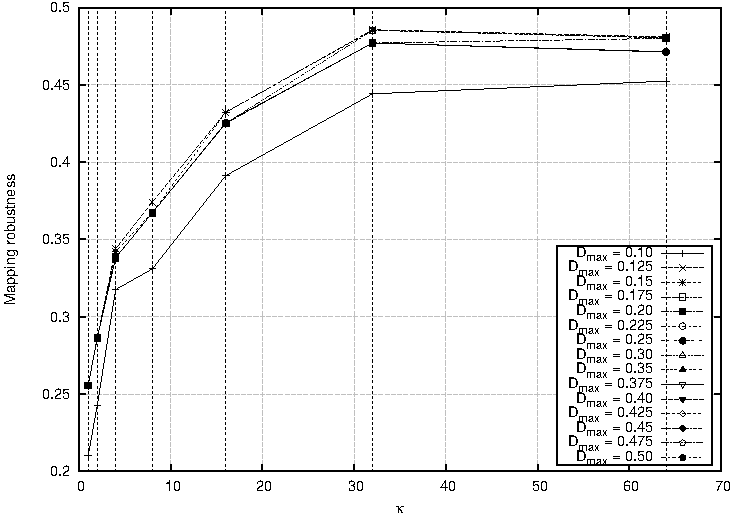
\includegraphics[width=.9\textwidth]{figures/web/longtail/fig_robustness}
  \caption{Plot of profile mapping robustness for varying $\kappa$.}
  \label{fig:robustness}
\end{figure}

\subsubsection{Detection accuracy}
\label{web:longtail:eval:detection}
Having studied the effects of profile clustering and varying values
for $\kappa$ upon the robustness of the profile mapping $f$, a
separate experiment was conducted in order to evaluate the detection
accuracy of a web application anomaly detector incorporating $\kb$,
the global knowledge base constructed in the previous experiments. In
particular, the goal of this experiment is to demonstrate that an
anomaly detector equipped with a global knowledge base exhibits an
improved detection accuracy in the presence of training data scarcity.

The data used in this experiment was a subset of the full dataset
described above, and was completely disjoint from the one used to
construct the global knowledge base and its indices.  It consisted of
220 unique real-world web applications, 8,402 unique resource paths,
7,648 distinct parameters, and 55,290,532 \ac{HTTP}\index{HTTP}
requests.

The intended threat model is that of an attacker attempting to
compromise the confidentiality or integrity of data exposed by a web
application by injecting malicious code in request parameters.

\begin{note}[Threat model]
  Although the anomaly detector used in this study is capable of
  detecting more complex session-level anomalies, we restrict the
  threat model to request parameter manipulation because we do not
  address session profile clustering.
\end{note}

To establish a worst-case bound on the detection accuracy of the
system, profiles for each observed request parameter were deliberately
undertrained to artificially induce a scarcity of training data for
\emph{all} parameters.  That is, for each value of
$\kappa=1,2,4,8,16,32,64$, the anomaly detector prematurely terminated
profile training after $\kappa$ samples, and then used the
undertrained profiles to query $\kb$.  The resulting global profiles
were then substituted for the undertrained profiles and evaluated
against the rest of the dataset.  The sensitivity of the system was
varied over the interval $\left[0,1\right]$, and the resulting
\ac{ROC}\index{ROC} curves for each $\kappa$ are plotted in
Figure~\ref{fig:roc}.

As one can clearly see, low values of $\kappa$ result in the selection
of global profiles that do not accurately model the behavior of the
undertrained parameters. As $\kappa$ increases, however, the quality
of the global profiles returned by the querying process increases as
well.  In particular, this increase in quality closely follows the
mapping robustness plot presented in Figure~\ref{fig:robustness}.  As
predicted, setting $\kappa=32,64$ leads to fairly accurate global
profile selection, with the resulting \ac{ROC}\index{ROC} curves
approaching that of fully-trained profiles.  This means that even if
the component of a web application has received only a few requests
(i.e., 64), by leveraging a global knowledge base it is possible to
achieve effective attack detection.  As a consequence, our approach
can improve the effectiveness of real-world web application firewalls
and web application anomaly detection systems.

Clearly, the detection accuracy will improve as more training samples
(e.g., 128, 256) become available. However, the goal of this
experiment was to evaluate such an improvement with a very limited
training set, rather than showing the detection maximum accuracy
achievable. From these results, we conclude that for appropriate
values of $\kappa$, the use of a global knowledge base can provide
reasonably accurate detection performance even in the presence of
training data scarcity.

\begin{figure}[t]
  \centering
  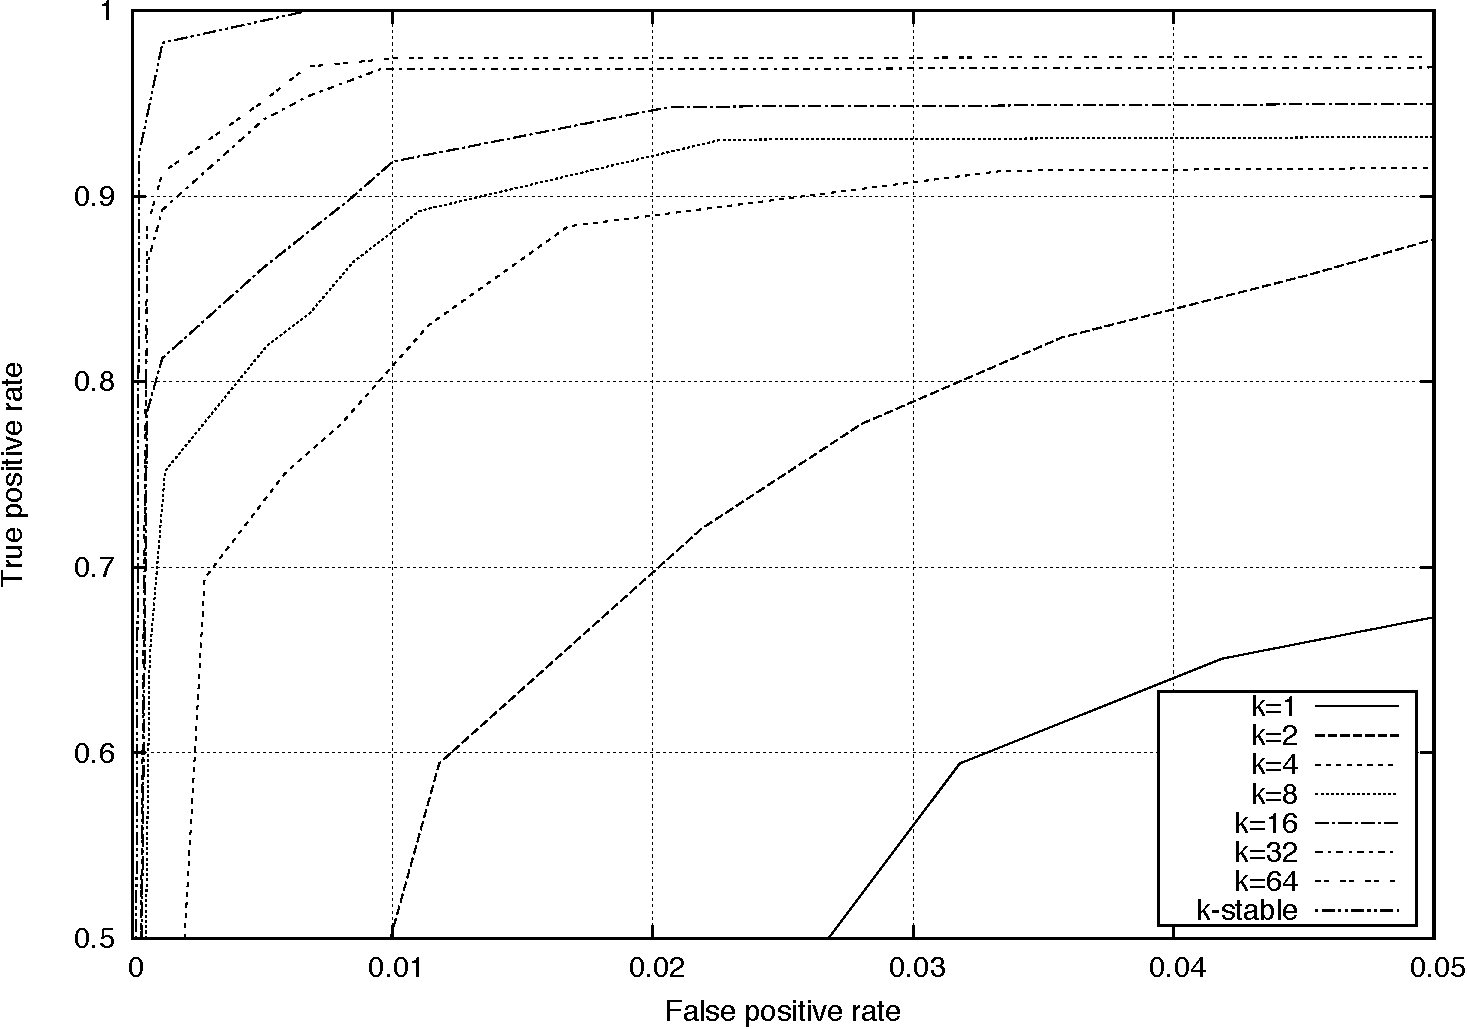
\includegraphics[width=.9\textwidth]{figures/web/longtail/fig_roc}
  \caption{Global profile ROC curves for varying $\kappa$. In the presence
    of severe undertraining ($\kappa \ll \kappa_{\text{stable}}$), the
    system is not able to recognize most attacks and also reports
    several false positives. However, as $\kappa$ increases, detection
    accuracy improves, and approaches that of the well-trained case
    ($\kappa=\kappa_{\text{stable}}$).}
  \label{fig:roc}
  \vspace*{-.5cm}
\end{figure}

One concern regarding the substitution of global profiles for local
request parameters is that a global profile that was trained on
another web application may not detect valid attacks against the
undertrained parameter.  Without this technique, however, recall that
a learning-based web application anomaly detector would otherwise have
no effective model whatsoever, and therefore the undertrained
parameter would be unprotected by the detection system (i.e., zero
true positive rate).  Furthermore, the \ac{ROC}\index{ROC} curves
demonstrate that while global profiles are in general not as precise
as locally-trained models, they do provide a significant level of
detection accuracy.

\begin{note}
  If global profiles were found to be as accurate as local profiles,
  this would constitute an argument against anomaly detection itself.
\end{note}

More precisely, with $\kappa = 1$, undertraining\index{undertraining} condition and system
off, only 67.5\% of the attacks are detected, overall, with around 5\%
of false positives. On the other hand, with $\kappa = 64$
(undertraining\index{undertraining} and system on), more than 91\% of the attacks are
detected with less than 0.2\% of false positives (\emph{vs.}, 0.1\% of
false positives in the case of no undertraining\index{undertraining} and system off).
Therefore, we conclude that, assuming no mistrust among the parties
that share the global knowledge base, our approach is a useful
technique to apply in the presence of undertrained models and, in
general, in the case of training data scarcity. Note that the last
assumption is often satisfied because one physical deployment (e.g.,
one server protected by our system) typically hosts several web
applications under the control of the same system administrator or
institution.

Therefore, we conclude that our approach is a useful technique to
apply in the presence of undertrained models and, in general, in case
of training data scarcity.

\begin{note}[Configuration parameters]
  Our methods provide explicit guidance, based on the training data of
  the particular deployment, to choose the value of the only parameter
  required to trade off accuracy \emph{vs.} length of the training
  phase. In addition, the ``goodness'' of the approach with respect to
  different choices of such a parameter is evaluated on real-world
  data in Section 4.

  In particular, the ROC curve shows how the sampling size ($\kappa$)
  affects the detection accuracy, thus offer some guidance to the
  user. In addition, Figure 8 shows that the system stabilizes for
  $\kappa > 32$, thus some more guidance about ``what is a good
  value'' is given.
\end{note}

\section{Addressing Changes in Web Applications}
\label{web:conceptdrift}
In this section, we describe our
proposal~\citep{2009_maggi_robertson_kruegel_vigna} to cope with
\ac{FP} due to changes in the modeled web applications. Recall that
detection is performed under the assumption that attacks cause
significant changes (i.e., anomalies) in the application
behavior. Thus, any activity that does not fit the expected, learned
models is flagged as malicious. This is true regardless of the type of
system activity, thus it holds for other types of \acp{IDS}\index{IDS}
than web-based ones.

In particular, one issue that has not been well-studied is the
difficulty of adapting to changes in the behavior of the protected
applications. This is an important problem because today's web
applications are user-centric. That is, the demand for new services
causes continuous updates to an application's logic and its
interfaces.

Our analysis, described in Section~\ref{web:conceptdrift:motivation},
reveals that significant changes in the behavior of web applications
are frequent. We refer to this phenomenon as \emph{web application
  concept drift}. In the context of anomaly-based detection, this
means that legitimate behavior might be misclassified as an attack
after an update of the application, causing the generation of false
positives. Normally, whenever a new version of an application is
deployed in a production environment, a coordinated effort involving
application maintainers, deployment administrators, and security
experts is required. That is, developers have to inform administrators
about the changes that are rolled out, and the administrators have to
update or re-train the anomaly models accordingly. Otherwise, the
amount of \acp{FP}\index{FP} will increase
significantly. In~\citep{2009_maggi_robertson_kruegel_vigna} we
describe a solution that makes these tedious tasks unnecessary. Our
technique examines the responses (\ac{HTML}\index{HTML} pages) sent by
a web application. More precisely, we check the forms and links in
these pages to determine when new elements are added or old ones
removed. This information is leveraged to recognizes when anomalous
inputs (i.e., \ac{HTTP}\index{HTTP} requests) are due to previous,
legitimate updates ---changes--- in a web application. In such cases,
\acp{FP}\index{FP} are suppressed by automatically and selectively
re-training models. Moreover, when possible, model parameters can be
automatically updated without requiring any re-training.

\begin{note}[Re-training]
  Often, a complete re-training of all the models is expensive in
  terms of time; typically, it requires $O(P)$ where $P$ represents
  the number of \ac{HTTP}\index{HTTP} messages required to train a
  model. More importantly, such re-training is not always feasible
  since new, attack-free training data is unlikely to be available
  immediately after the application has changed. In fact, to collect a
  sufficient amount of data the new version of the application must be
  executed and real, legitimate clients have to interact with it in a
  controlled environment. Clearly, this task requires time and
  efforts. More importantly, those parts that have changed in the
  application must be known in advance.

  Our technique focuses on the fundamental problem of \emph{detecting}
  those parts of the application that have changed and that will cause
  \acp{FP}\index{FP} if no re-training is performed. Therefore, the
  technique is agnostic with respect to the specific training
  procedure, which is \ac{IDS}-specific and can be different from the
  one we propose.
\end{note}

The core of this contribution is the exploiting of
\ac{HTTP}\index{HTTP} responses, which we show to contain important
insights that can be effectively leveraged to update previously
learned models to take changes into account. The results of applying
our technique on real-world data demonstrate that learning-based
anomaly detectors can automatically \emph{adapt to changes}, and by
doing this, are able to reduce their \ac{FPR} without decreasing their
\ac{DR} significantly. Note that, in general, relying on HTTP
responses may lead to the issue of poisoning of the models used to
characterize them: this limitation is discussed in details in
Section~\ref{web:conceptdrift:design:discussion} in comparison with
the advantages provided by our technique.

In Section~\ref{web:conceptdrift:motivation} the problem of concept
drift in the context of web applications is detailed. In addition, we
provide evidence that it occurs in practice, motivating why it is a
significant problem for deploying learning-based anomaly detectors in
the real world. The core of our contribution is described in
Section~\ref{web:conceptdrift:design} where we detail the technique
based on \ac{HTTP}\index{HTTP} response models that can be used to
distinguish between legitimate changes in web applications and
web-based attacks. A version of \webanomaly incorporating these
techniques has been evaluated over an extensive real-world data set,
demonstrating its ability to deal with web application concept drift
and reliably detect attacks with a low false positive rate. The
results of this evaluation are discussed in
Section~\ref{web:conceptdrift:eval}.

\subsection{Web Application Concept drift}
\label{web:conceptdrift:motivation}
In this section the notion of web application concept drift is defined. We rely upon the generalized model of learning-based anomaly detectors of web attacks described in Section~\ref{web:intro:ad}. Secondly, evidence that concept drift is a problem that exists in the real world is provided to motivate why it should be addressed.

\subsubsection{Changes in Web Applications' Behavior}
\label{web:conceptdrift:motivation:dynamic}
In machine learning, changes in the modeled behavior are known as \emph{concept drift}~\citep{concept-drift:conference}. Intuitively, the \emph{concept} is the modeled phenomenon; in the context of anomaly detection it may be the structure of requests to a web server, the recurring patterns in the payload of network packets, etc. Thus, variations in the main features of the phenomena under consideration result in changes, or \emph{drifts}, in the \emph{concept}. In some sense, the \emph{concept} corresponds to the normal web application behavior (see also Definition~\ref{def:system-behavior}).

Although the generalization and abstraction capabilities of modern learning\hyp{}based anomaly detectors are resilient to noise (i.e., small, legitimate variations in the modeled behavior), concept drift is difficult to detect and to cope with~\citep{concept-drift:journal}. The reason is that the parameters of the models may stabilize to different values. For example, the string length model described in Section~\ref{host:improving:exec-models} ---and also used in \webanomaly--- learns the sample mean and variance of the string lengths that are observed during training. In \webanomaly, during detection, the Chebyshev\index{Chebyshev} inequality is used to detect strings with lengths that significantly deviate from the mean, taking into account the observed variance. As shown in Section~\ref{host:improving:accuracy}, the variance allows to account for small differences in the lengths of strings that will be considered normal.

On the other hand, the mean and variance of the string lengths can completely change because of legitimate and permanent modifications in the web application. In this case, the normal mean and variance will stabilize, or drift, to different values. If appropriate re-training or manual updates are not performed, the model will classify benign, new strings as anomalous. These examples allow us to better define the web application concept drift.

\begin{definition}[Web Application Concept Drift]
  The \emph{web application concept drift} is a permanent modification of the \emph{normal web application behavior}.
\end{definition}

\noindent Since the behavior of a web application is derived from the system activity $\mathbb{I}$ during normal operation, a permanent \emph{change} in $\mathbb{I}$ causes the concept drift. Changes in web applications can manifest themselves in several ways. In the context of learning-based detection of web attacks, those changes can be categorized into three groups: \emph{request} changes, \emph{session} changes, and \emph{response} changes.

\paragraph{Request changes} Changes in requests occur when an application is upgraded to handle different \ac{HTTP}\index{HTTP} requests. These changes can be further divided into two groups: \emph{parameter value} changes and \emph{request structure} changes. The former involve modifications of the actual value of the parameters, while the latter occur when parameters are \emph{added} or \emph{removed}. Parameter \emph{renaming} is the result of removal plus addition.

\begin{example}[Request change]
  A new version of a web forum introduces internationalization (I18N) and localization (L10N). Besides handling different languages, I18N and L10N allow several types of strings to be parsed as valid dates and times. For instance, valid strings for the \texttt{datetime} parameter are \texttt{`3 May 2009 3:00'}, \texttt{`3/12/2009'}, \texttt{`3/12/2009 3:00 PM GMT-08'}, \texttt{`now'}. In the previous version, valid date-time strings had to conform to the regular expression \texttt{`[0-9]\{1,2\}/[0-9]\{2\}/[0-9]\{4\}'}. A model with good generalization properties would learn that the field \texttt{datetime} is composed of numbers and slashes, with no spaces. Thus, other strings such as \texttt{`now'} or \texttt{`3/12/2009 3:00 PM GMT-08'} would be flagged as anomalous. Also, in our example, \texttt{tz} and \texttt{lang} parameters have been added to take into account time zones and languages. To summarize, the new version introduces two classes of changes. Clearly, the parameter domain of \texttt{datetime} is modified. Secondly, new parameters are added.
\end{example}

Changes in \ac{HTTP}\index{HTTP} requests directly affect the request models:

\begin{enumerate}
\item parameter value changes affect any models that rely on the parameters' \emph{values} to extract features. For instance, consider two of the models used in the system described in \citep{kruegel:jcn2005:webanomaly}: $\mchar$ and $\mstruct$. The former models the strings' character distribution by storing the frequency of all the symbols found in the strings during training, while the latter models the strings' structure as a stochastic grammar, using a \ac{HMM}. In the aforementioned example, the I18N and L10N introduce new, legitimate values in the parameters; thus, the frequency of numbers in $\mchar$ changes and new symbols (e.g., \texttt{`-'}, \texttt{`[a-zA-Z]'} have to be taken into account. It is straightforward to note that $\mstruct$ is affected in terms of new transitions introduced in the \ac{HMM}\index{HMM} by the new strings.

\item Request structure changes may affect any type of request model, regardless of the specific characteristics. For instance, if a model for a new parameter is missing, requests that contain that parameter might be flagged as anomalous.
\end{enumerate}

\paragraph{Session changes} Changes in sessions occur whenever resource path sequences are \emph{reordered}, \emph{inserted}, or \emph{removed}. Adding or removing application modules introduces changes in the session models. Also, modifications in the application logic are reflected in the session models as reordering of the resources invoked.

\begin{example}[Session change]
  A new version of a web-based community software grants read-only access to \emph{anonymous} users (i.e., without authentication), allowing them to display contents previously available to subscribed users only. In the old version, legitimate sequences were $\langle$\texttt{/site, /auth, /blog}$\rangle$ or $\langle$\texttt{/site, /auth, /files}$\rangle$, where \texttt{/site} indicates the server-side resource that handles the public site, \texttt{/auth} is the authentication resource, and \texttt{/blog} and \texttt{/files} were formerly private resources. Initially, the probability of observing $\mathtt{/auth}$ before \texttt{/blog} or \texttt{/files} is close to one (since users need to authenticate before accessing private material). This is no longer true in the new version, however, where \texttt{/files|/blog|/auth} are all possible after \texttt{/site}.
\end{example}

Changes in sessions impact all models that rely on the sequence of resources that are invoked during the normal operation of an application. For instance, consider the model $\msess$ described in \citep{kruegel:jcn2005:webanomaly}, which builds a probabilistic finite state automaton that captures sequences of \emph{resource paths}. New arcs must be added to take into account the changes mentioned in the above example. These types of models are sensitive to strong changes in the session structure and should be updated accordingly when they occur.

\paragraph{Response changes} Changes in responses occur whenever an application is upgraded to produce different responses. Interface redesigns and feature addition or removal are example causes of changes in the responses. Response changes are common and frequent, since page updates or redesigns often occur in modern websites.

\begin{example}[Response change]
  A new version of a video sharing application introduces Web 2.0 features into the user interface, allowing for the modification of user interface elements without refreshing the entire page.  In the old version, relatively few nodes of documents generated by the application contained client-side code. In the new version, however, many nodes of the document contain event handlers to trigger asynchronous requests to the application in response to user events. Thus, if a response model is not updated to reflect the new structure of such documents, a large of number of false positives will be generated due to \emph{legitimate} changes in the characteristics of the web application responses.
\end{example}

\subsubsection{Concept Drift in the Real World}
\label{web:conceptdrift:motivation:prevalence}
To understand whether concept drift is a relevant issue for real-world websites, we performed three experiments.  For the first experiment, we monitored 2,264 public websites, including the \textsf{Alexa} Top 500's and other sites collected by querying \textsf{Google} with popular terms extracted from the \textsf{Alexa} Top 500's. The goal was to identify and quantify the changes in the forms and input fields of popular websites at large. This provides an indication of the frequency with which real-world applications are updated or altered.

\paragraph{First Experiment: Frequency of Changes}
Once every hour, we visited one page for each of the 2,264
websites. In total, we collected 3,303,816 pages, comprising more than
1,390 snapshots for each website, between January 29 and April 13,
2009. One tenth of the pages were manually selected to have a
significant number of forms, input fields, and hyperlinks with
\texttt{GET} parameters. By doing this, we gathered a considerable
amount of information regarding the \ac{HTTP}\index{HTTP} messages
generated by some applications. Examples of these pages are
registration pages, data submission pages, or contact form pages. For
the remaining websites, we simply used their home pages. Note that,
the pages we selected may not be fully representative of the whole
website. To overcome this limitation and to further confirm our
intuition, we performed a more detailed experiment --- described in
Section~\ref{web:concept-drift:motivation:third} --- on the source
code of large, real-world web applications.

For each website $w$, each page sample crawled at time $t$ is
associated with a tuple $|F|^{(w)}_{t}, |I|^{(w)}_{t}$, the
cardinality of the sets of forms and input fields, respectively. By
doing this, we collected samples of the variables $|F|^{w} =
|F|^{w}_{t_{1}}, \dots, |F|^{w}_{t_{n}}$, $|I|^{w} = |I|^{w}_{t_{1}},
\dots, |I|^{w}_{t_{n}}$, with $0 < n <
1,390$. Figure~\ref{fig:website-features-changes} shows the relative
frequency of the variables

\begin{eqnarray*}
  X_{I} &=& \stdev(|I|^{(w_{1})}), \dots, \stdev(|I|^{(w_{k})})\\
  X_{F} &=& \stdev(|F|^{(w_{1})}), \dots, \stdev(|F|^{(w_{k})}).
\end{eqnarray*}

This demonstrates that a significant amount of websites exhibit
variability in the response models, in terms of elements modified in
the pages, as well as request models, in terms of new forms and
parameters. In addition, we estimated the expected time between
changes of forms and inputs fields, $E[T_{F}]$ and $E[T_{I}]$,
respectively. In terms of forms, 40.72\% of the websites drifted
during the observation period. More precisely, 922 out of 2,264
websites have a finite $E[T_{F}]$. Similarly, 29.15\% of the websites
exhibited drifts in the number of input fields, i.e., $E[T_{I}] <
+\infty$ for 660 websites. Figure~\ref{fig:website-features-changes}
shows the relative frequency of
\subref{subfig:website-forms-change-time} $E[T_{F}]$, and
\subref{subfig:website-inputs-change-time}
$E[T_{I}]$. $E[T_{F}]$. This confirms that a non-negligible portion of
the websites exhibit significantly frequent changes in the responses.

\begin{figure}[t]
  \centering
  
  \subfloat[Changes of
  forms.]{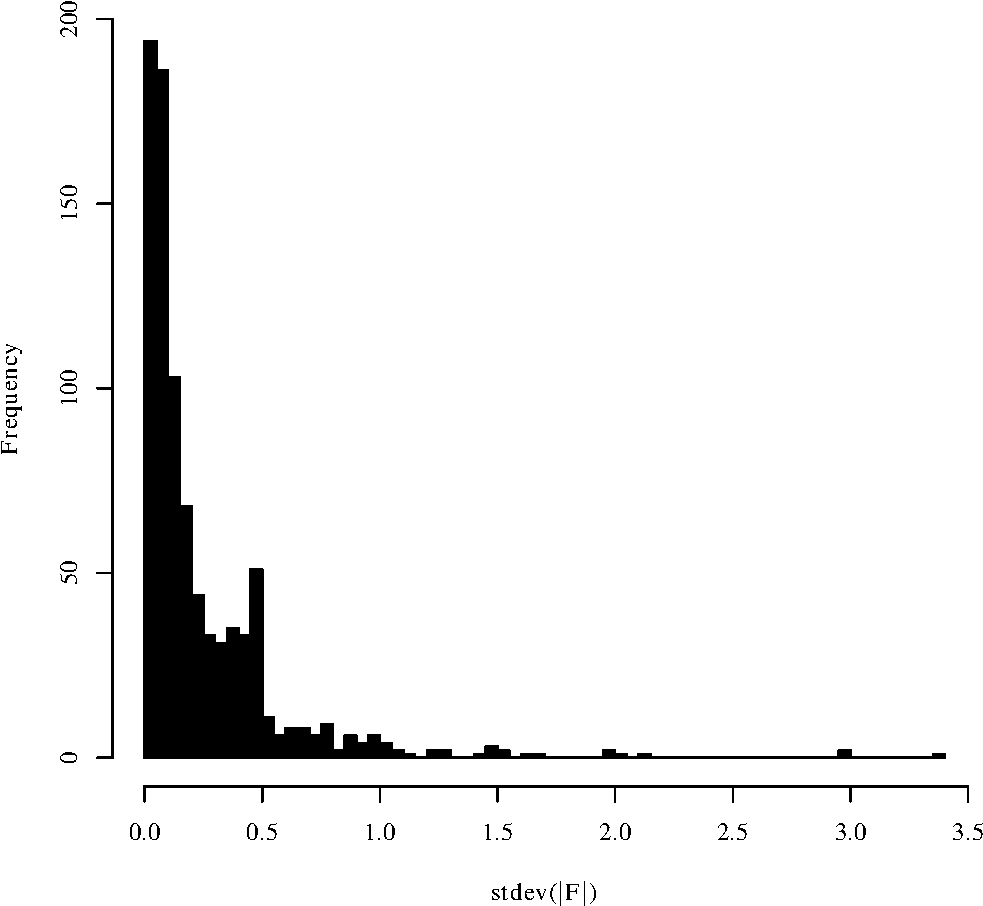
\includegraphics[width=.5\textwidth]{figures/web/conceptdrift/fig_stddev_forms}\label{subfig:website-forms-changes}}
  \subfloat[Avg. time between changes in
  $|F|$.]{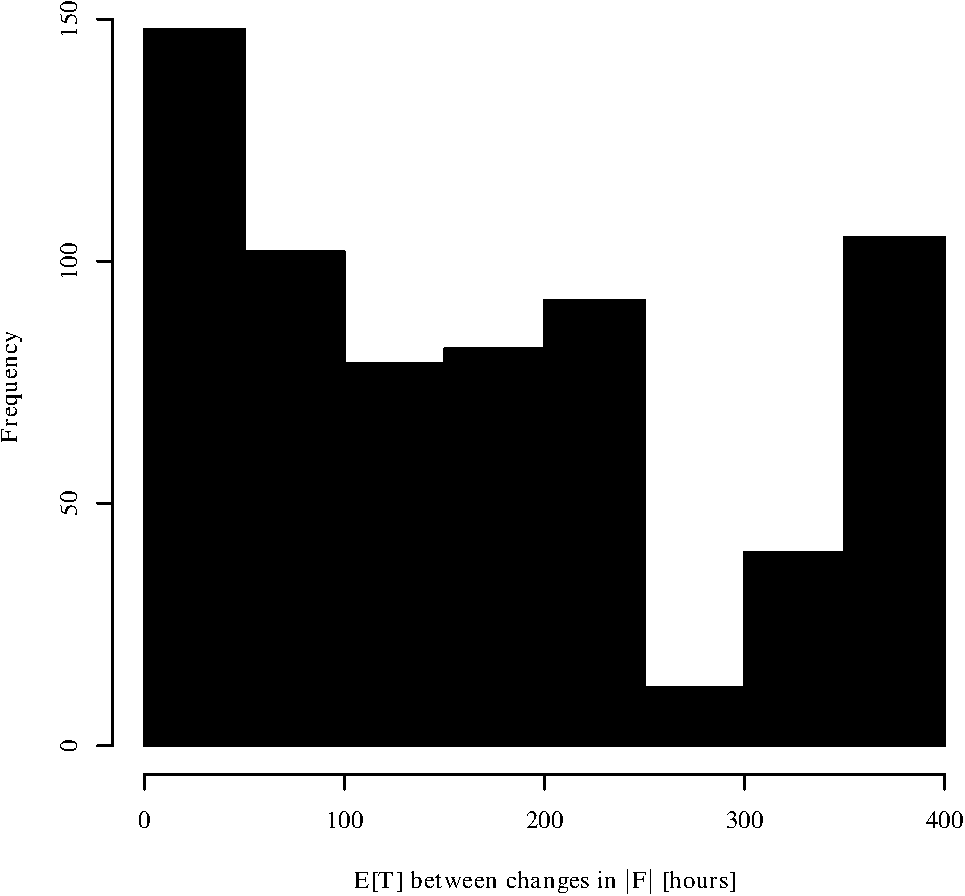
\includegraphics[width=.5\textwidth]{figures/web/conceptdrift/fig_atf}\label{subfig:website-forms-change-time}}\\

  \subfloat[Changes of
  inputs.]{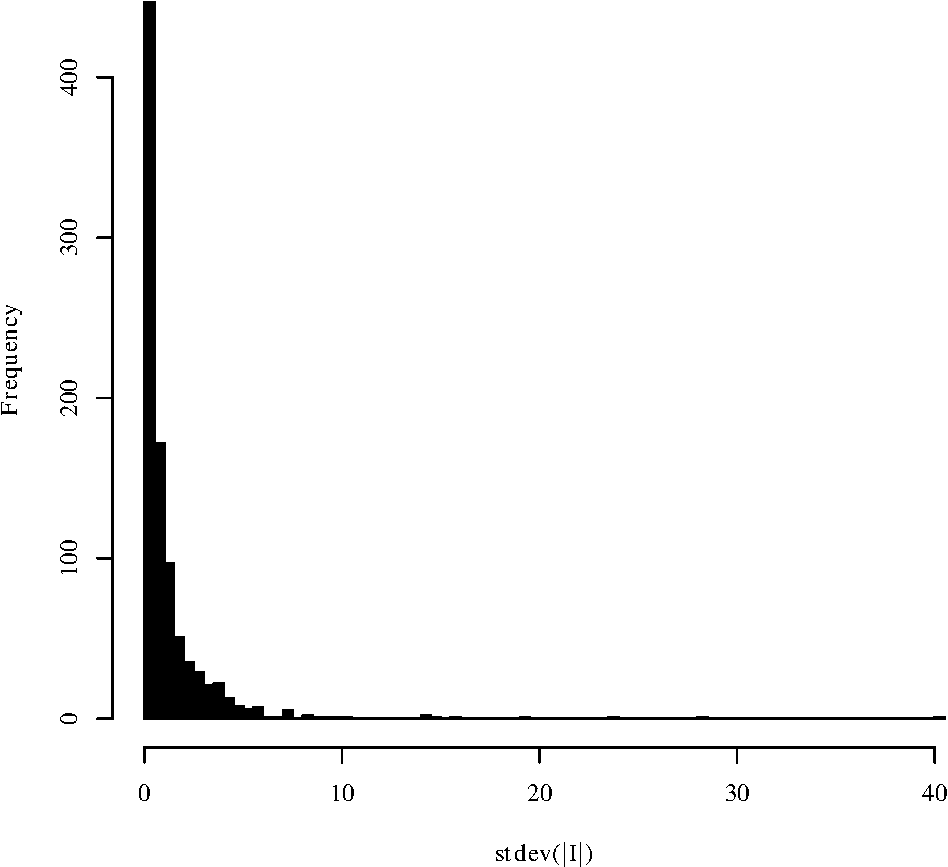
\includegraphics[width=.5\textwidth]{figures/web/conceptdrift/fig_stddev_inputs}\label{subfig:website-inputs-changes}}
  \subfloat[Avg. time between changes in
  $|I|$]{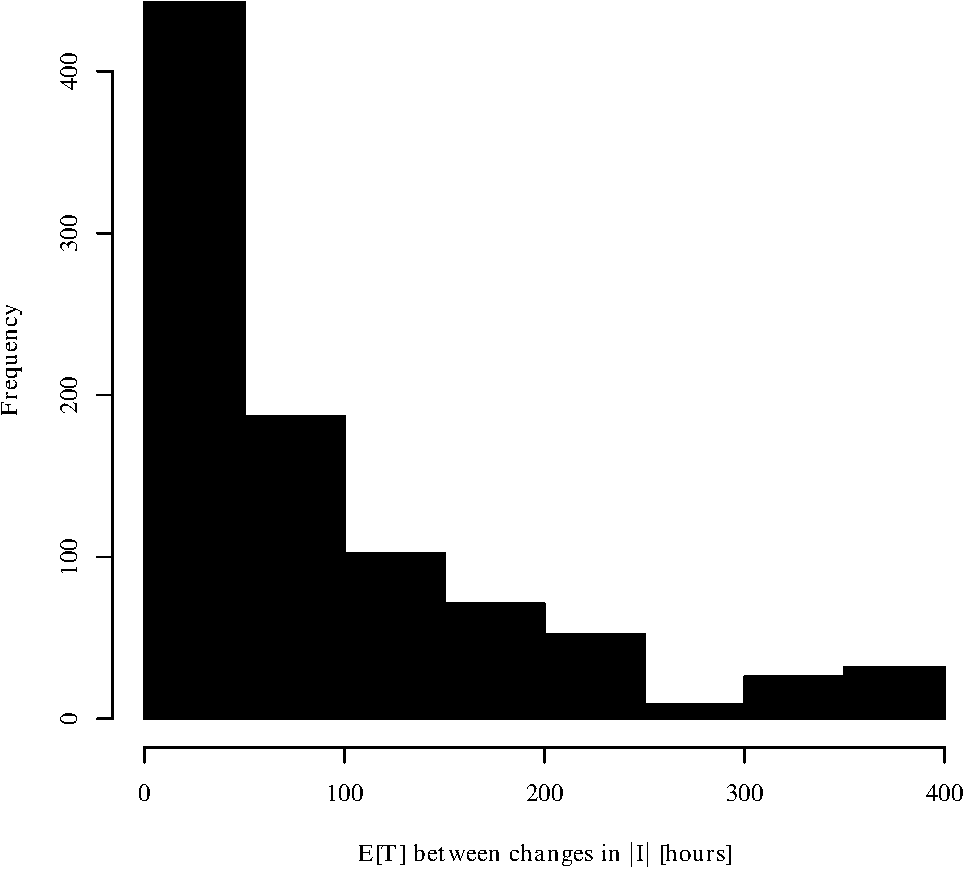
\includegraphics[width=.5\textwidth]{figures/web/conceptdrift/fig_ati}\label{subfig:website-inputs-change-time}}

  \caption{Relative frequency of the standard deviation of the number
    of forms \protect\subref{subfig:website-forms-changes} and input
    fields \protect\subref{subfig:website-inputs-changes}. Also, the
    distribution of the expected time between changes of forms
    \protect\subref{subfig:website-forms-change-time} and input fields
    \protect\subref{subfig:website-inputs-change-time} are plotted. A
    non-negligible portion of the websites exhibits changes in the
    responses. No differences have been noticed between home pages and
    manually-selected pages.}
  \label{fig:website-features-changes}
  \vspace*{-.65cm}
\end{figure}

\paragraph{Second Experiment: Type of Changes}
We monitored in depth three large, data-centric web applications over several months: \textsf{Yahoo!  Mail}, \textsf{YouTube}, and \textsf{MySpace}. We dumped \ac{HTTP}\index{HTTP} responses captured by emulating user interaction using a custom, scriptable web browser implemented with \textsf{Html\hyp{}Unit}. Examples of these interactions are as follows: visit the home page, login, browse the inbox, send messages, return to the home page, click links, log out. Manual inspection revealed some major changes in \textsf{Yahoo! Mail}. For instance, the most evident change consisted of a set of new features added to the search engine (e.g., local search, refined address field in maps search), which manifested themselves as new parameters found in the web search page (e.g. to take into account the country or the ZIP code). User pages of \textsf{YouTube} were significantly updated with new functionalities between 2008 and 2009. For instance, the new version allows users to rearrange widgets in their personal pages. To account for the position of each element, new parameters are added to the profile pages and submitted asynchronously whenever the user drags widgets within the layout. The analysis on \textsf{MySpace} did not reveal any significant change. The results of these two experiments show that changes in server-side applications are common. More importantly, these modifications often involve the way user data is represented, handled, and manipulated.

\paragraph{Third Experiment: Abundance of Code Change}
\label{web:concept-drift:motivation:third}
We analyzed changes in the requests and sessions by inspecting the
code repositories of three of the largest, most popular open-source
web applications: \textsf{WordPress}, \textsf{Movable Type}, and
\textsf{PhpBB}. The goal was to understand whether upgrading a web
application to a newer release results in significant changes in the
features that are used to determine its behavior. In this analysis, we
examined changes in the source code that affect the manipulation of
\ac{HTTP}\index{HTTP} responses, requests, and session data. We used
\textsf{StatSVN}, an open-source tool for tracking and visualizing the
activity of \ac{SVN}\index{SVN} repositories (e.g., the number of
lines changed or the most active developers). We modified
\textsf{StatSVN} to incorporate a set of heuristics to compute
approximate counts of the lines of code that, directly or indirectly,
manipulate \ac{HTTP}\index{HTTP} session, request or response data. In
the case of \ac{PHP}\index{PHP}, examples representative of such lines
include, but are not limited to,
\texttt{\_REQUEST|\_SESSION|\_POST|\_GET|session\_[a-z]+|http\_|strip\_tags|addslashes}. In
order to take into account data manipulation performed through library
functions (e.g., \textsf{WordPress}' custom \texttt{Http} class), we
also generated application-specific code patterns by manually
inspecting and filtering the core
libraries. Figure~\ref{fig:code-changes} shows, over time, the lines
of code in the repositories of \textsf{PhpBB}, \textsf{WordPress}, and
\textsf{Movable Type} that manipulate \ac{HTTP}\index{HTTP} responses,
requests and, sessions. These results show the presence of significant
modifications in the web application in terms of relevant lines of
code added or removed. More importantly, such modifications affect the
way \ac{HTTP}\index{HTTP} data is manipulated and, thus, impact
request, response or session models.

\begin{figure}[p]
  \centering
  \subfloat[\textsf{PhpBB}]{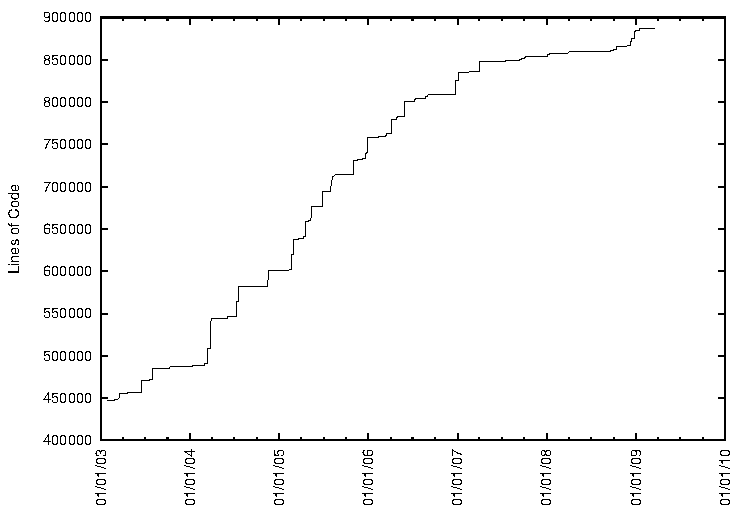
\includegraphics[width=.7\textwidth]{figures/web/conceptdrift/fig_phpbb_svn_loc}\label{subfig:phpbb-code-changes}}\\
  \subfloat[\textsf{WordPress}]{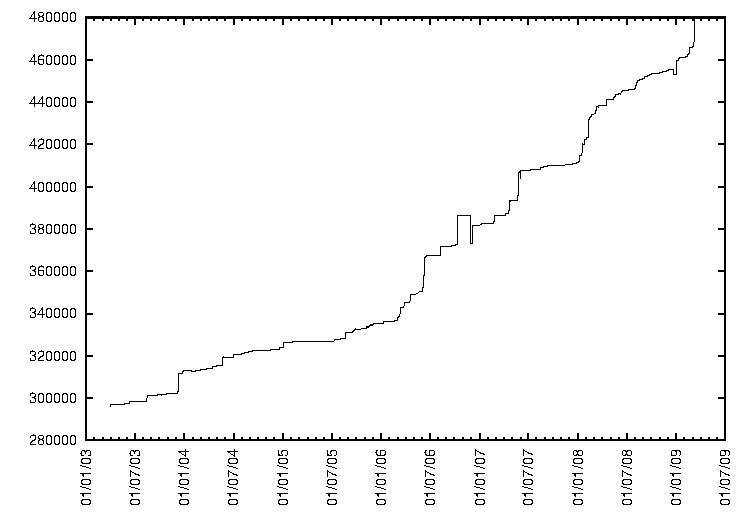
\includegraphics[width=.7\textwidth]{figures/web/conceptdrift/fig_wp_svn_loc}\label{subfig:wordpress-code-changes}}\\
  \subfloat[\textsf{Movable Type}]{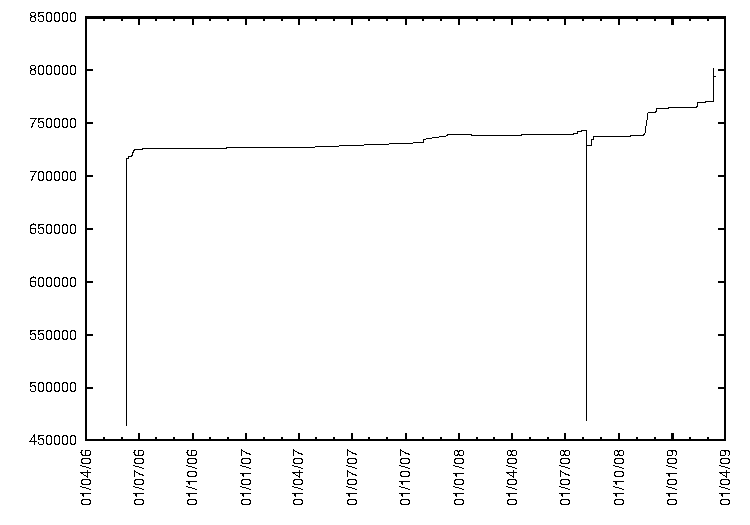
\includegraphics[width=.7\textwidth]{figures/web/conceptdrift/fig_mtos_svn_loc}\label{subfig:movabletype-code-changes}}

  \caption{Lines of codes in the repositories of \textsf{PhpBB}, \textsf{WordPress}, and \textsf{Movable Type}, over time. Counts include only the code that manipulates \ac{HTTP}\index{HTTP} responses, requests and sessions.}
  \label{fig:code-changes}
  \vspace*{-.65cm}
\end{figure}

The aforementioned experiments confirm that the class of changes we described in Section~\ref{web:conceptdrift:motivation:dynamic} is common in real-world web applications. Therefore, anomaly detectors for web applications must incorporate procedures to prevent false alerts due to concept drift. In particular, a mechanism is needed to discriminate between legitimate and malicious changes, and respond accordingly. Note that, this somehow coincides with the original definition of \ac{ID} (i.e., distinguishing among normal \emph{vs.} malicious activity); however, our focus is to recognizes changes in the application \emph{activity} that could lead to concept drift as opposed to spotting out changes in the application \emph{behavior} (i.e., \ac{ID}).

\subsection{Addressing concept drift}
\label{web:conceptdrift:design}
In this section, a technique is presented to distinguish between legitimate changes in web application behavior and evidence of malicious behavior.

\subsubsection{Exploiting HTTP responses}
\label{web:conceptdrift:design:oracle}
An \ac{HTTP}\index{HTTP} response is composed of a header and a body. Under the hypothesis of content-type \texttt{text/html}, the body of \ac{HTTP}\index{HTTP} responses contains a set of links $L_i$ and forms $F_i$ that refer to a set of target resources.  Each form also includes a set of input fields $I_i$.  In addition, each link $l_{i,j}\in L_i$ and form $f_{i,j}\in F_i$ has an associated set of parameters.

A request $q_{i}$ to a resource $r_{i}$ returns a response $resp_{i}$. From $resp_{i}$ the client follows a link $l_{i,j}$ or submits a form $f_{i,j}$.  Either of these actions generates a new \ac{HTTP}\index{HTTP} request to the web application with a set of parameter key-value pairs, resulting in the return of a new \ac{HTTP}\index{HTTP} response to the client, $r_{i+1}$, the body of which contains a set of links $L_{i+1}$ and forms $F_{i+1}$. According to the specifications of the \ac{HTTP}\index{HTTP}, this process continues until the session has ended (i.e., either the user has explicitly logged out, or a timeout has occurred). We then define:

\begin{definition}[Candidate Resource Set]
  Given a resource $r$ within a web application, the \emph{candidate resource set} of $r$ is defined as:

  \begin{eqnarray*}
    \mathrm{candidates(r)} & := & L_{r} \cup F_{r} = \\
                           & = & \{l_{1}, l_{2}, \dots, l_{N}\} \cup\\
                           &    & \{f_{1}, f_{2}, \dots, f_{M}\}.
  \end{eqnarray*}

  \noindent where:

  \begin{itemize}

  \item $l_{(\cdot)} := resp.\mathtt{a_{(\cdot)}.href}$,

  \item $f_{(\cdot)} := resp.\mathtt{form_{\mathrm{(\cdot)}}.action}$,

  \item $resp.$ is the \texttt{plain/text} body of the response $resp$,

  \item $resp.$\texttt{<element>}$_{\mathrm{(\cdot)}}.$\texttt{<attribute>}
    is the content of the attribute,

  \item \texttt{<attribute>}, of the \ac{HTML}\index{HTML}
    \texttt{<element>}$_{(\cdot)}$.
  \end{itemize}
\end{definition}

Our key observation is that, at each step of a web application session, a subset of the \emph{potential} target resources is given exactly by the content of the current resource.  That is, given $r_i$, the associated sets of links $L_i$ and forms $F_i$ directly encode a significant sub-set of the possible $r_{i+1}$.  Furthermore, each link $l_{i,j}$ and form $f_{i,j}$ indicates a precise set of expected parameters and, in some cases, the set of legitimate values for those parameters that can be provided by a client.

Consider a hypothetical banking web application, where the current resource $r_i=\mathtt{/account}$ presented to a client is an account overview. The response $resp_{i}$ may contain:

\begin{html}
<body class="account">
  /* ... */

  <form action="/search" method="get">
    <input name="term" type="text" value="Insert term" />
    <input type="submit" value="Search!" />
  </form>  

  <h1><a href="/account/transfer">Transfer funds</a></h1>
  <a href="/account/transfer/submit">Submit transfer</a>

  /* ... */

  <tr><td><a href="/account/history?aid=328849660322">See details</a></td></tr>
  <tr><td><a href="/account/history?aid=446825759916">See details</a></td></tr>

  /* ... */

  <a href="/logout">Logout</a>

  /* ... */

  <h2>Feedback on this page?</h2>
  <form action="/feedback" method="post" class="feedback-form">
    <select name="subject">
      <option>General</option>
      <option>User interface</option>
      <option>Functionality</option>
    </select>
    <textarea name="message" />
    <input type="submit" />
  </form>

  /* - */
</body>
\end{html}

\noindent containing a set of links $L_{i}$, represented as their \ac{URL}\index{URL}, for instance:

\begin{displaymath}
  L_{i} =
  \left\{
    \begin{array}{l}
      \texttt{/account/history?aid=328849660322},\\
      \texttt{/account/history?aid=446825759916},\\
      \texttt{/account/transfer/submit},\\
      \texttt{/account/transfer},\\
      \texttt{/logout}
    \end{array}
  \right\}.
\end{displaymath}

\noindent Forms are represented as their target action. For instance: $F_{i} =\{$\texttt{/feedback}, \texttt{/search}$\}$.

From $L_i$ and $F_i$, we can deduce the set of legal candidate resources for the next request $r_{i+1}$.  Any other resource would, by definition, be a deviation from a legal session flow through the web application as specified by the application itself.  For instance, it would not be expected behavior for a client to directly access \texttt{/account/transfer/submit} (i.e., a resource intended to submit an account funds transfer) from $r_i$.  Furthermore, for the resource \texttt{/account/history}, it is clear that the web application expects to receive a single parameter \texttt{aid} with an account number as an identifier.

In the case of the form with target \texttt{/feedback}, let the associated input elements be:

\begin{html}
    <select name="subject">
      <option>General</option>
      <option>User interface</option>
      <option>Functionality</option>
    </select>
    <textarea name="message" />
\end{html}

It immediately follows that any invocation of the \texttt{/feedback} resource from $r_i$ should include the parameters \texttt{subject} and \texttt{message}.  In addition, the legal set of values for the parameter \texttt{subject} is given by enumerating the enclosed \texttt{<option~/>} tags. Valid values for the new \texttt{tz} and \texttt{datetime} parameters mentioned in the example of Section~\ref{web:conceptdrift:motivation:dynamic} can be inferred using the same algorithm. Any deviation from these specifications could be considered evidence of malicious behavior.

In this section we described why responses generated by a web application constitute a specification of the intended behavior of clients and the expected inputs to an application's resources.  As a consequence, when a change occurs in the interface presented by a web application, this will be reflected in the content of its responses.  Therefore, as detailed in the following section, an anomaly detection system can take advantage of response modeling to detect and adapt to changes in monitored web applications.

\subsubsection{Adaptive response modeling}
\label{web:conceptdrift:design:responses}
In order to detect changes in web application interfaces, the response modeling of \webanomaly has been augmented with the ability to build $L_{i}$ and $F_{i}$ from the \ac{HTML}\index{HTML} documents returned to a client. The approach is divided into two phases.

\paragraph{Extraction and parsing}
\label{web:conceptdrift:design:responses:extraction-parsing}
The anomaly detector parses each \ac{HTML}\index{HTML} document contained in a response issued by the web application to a client.  For each \texttt{<a~/>} tag encountered, the contents of the \texttt{href} attribute is extracted and analyzed.  The link is decomposed into tokens representing the protocol (e.g., \texttt{http}, \texttt{https}, \texttt{javascript}\index{JavaScript}, \texttt{mailto}), target host, port, path, parameter sequence, and anchor.  Paths are subject to additional processing; for instance, relative paths are normalized to obtain a canonical representation.  This information is stored as part of an abstract document model for later processing.

A similar process occurs for forms.  When a \texttt{<form~/>} tag is encountered, the \texttt{action} attribute is extracted and analyzed as in the case of the link \texttt{href} attribute.  Furthermore, any \texttt{<input~/>}, \texttt{<textarea~/>}, or \texttt{<select~/>} and \texttt{<option~/>} tags enclosed by a particular \texttt{<form~/>} tag are parsed as parameters to the corresponding form invocation.  For \texttt{<input~/>} tags, the \texttt{type}, \texttt{name}, and \texttt{value} attributes are extracted. For \texttt{<textarea~/>} tags, the \texttt{name} attribute is extracted.  Finally, for \texttt{<select~/>} tags, the \texttt{name} attribute is extracted, as well as the content of any enclosed \texttt{<option~/>} tags.  The target of the form and its parameters are recorded in the abstract document model as in the case for links.

\paragraph{Analysis and modeling}
\label{web:conceptdrift:design:responses:analysis-modeling}
The set of links and forms contained in a response is processed by the anomaly engine.  For each link and form, the corresponding target resource is compared to the existing known set of resources.  If the resource has not been observed before, a new model is created for that resource.  The session model is also updated to account for a potential transition from the resource associated with the parsed document and the target resource by training on the observed session request sequence.

For each of the parameters parsed from links or forms contained in a response, a comparison with the existing set of known parameters is performed.  If a parameter has not already been observed (e.g., the new \texttt{tz} parameter), a profile is created and associated with the target resource model.

Any values contained in the response for a given parameter are processed as training samples for the associated models.  In cases where the total set of legal parameter values is specified (e.g., \texttt{<select~/>} and \texttt{<option~/>} tags), the parameter profile is updated to reflect this.  Otherwise, the profile is trained on subsequent requests to the associated resource.

As a result of this analysis, the anomaly detector is able to adapt to changes in session structure resulting from the introduction of new resources.  In addition, the anomaly detector is able to adapt to changes in request structure resulting from the introduction of new parameters and, in a limited sense, to changes in parameter values.

\begin{figure}[t]
  \centering
  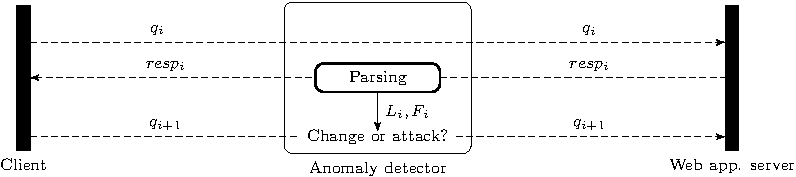
\includegraphics[width=\textwidth]{figures/web/conceptdrift/fig_design}

  \caption{A representation of the interaction between the client and the web application server, monitored by a learning-based anomaly detector. After request $q_{i}$ is processed, the corresponding response $resp_{i}$ is intercepted and link $L_{i}$ and forms $F_{i}$ are parsed to update the request models. This knowledge is exploited as a change detection criterion for the subsequent request $q_{i+1}$.}
  \label{fig:design}
  \vspace*{-.5cm}
\end{figure}

\subsubsection{Advantages and limitations}
\label{web:conceptdrift:design:discussion}
Due to the response modeling algorithm described in the previous section, an anomaly detector is able to automatically adapt to many common changes observed in web applications as modifications are made to the interface presented to clients.  Both changes in session and request structure such as those described in Section~\ref{web:conceptdrift:motivation:dynamic} can be accounted for in an automated fashion.

\begin{example}[I18N and L10N]
  The aforementioned modification is correctly handled as it consists in an addition of the \texttt{tz} parameter and a modification of the \texttt{datetime} parameter.
\end{example}

Furthermore, we claim that web application anomaly detectors that do not perform response modeling cannot reliably distinguish between anomalies caused by legitimate changes in web applications and those caused by malicious behavior.  Therefore, as will be shown in Section~\ref{web:conceptdrift:eval}, any such detector that solely monitors requests is more prone to false positives in the real world.

\medskip

\noindent Clearly, the technique relies upon the assumption that the web application has not been compromised.  Since the web application, and in particular the documents it generates, is treated as an oracle for whether a change has occurred, if an attacker were to compromise the application in order to introduce a malicious change, the malicious behavior would be learned as normal by the detector.  Of course, in this case, the attacker would already have access to the web application. However, modern anomaly detectors like \webanomaly observes all requests and responses to and from untrusted clients, therefore, any attack that would compromise response modeling would be detected and blocked.

\begin{example}
  An attacker could attempt to evade the anomaly detector by introducing a malicious change in the \ac{HTTP}\index{HTTP} responses and then exploits the change detection technique that would interpret the new malicious request as a legit change.

For instance, the attacker could incorporate a link that contain a parameter used to inject the attack vector. To this end, the attacker would have to gain control of the server by leveraging an existing vulnerability of the web application (e.g., a buffer overflow, a \ac{SQL}\index{SQL} injection). However, the \ac{HTTP}\index{HTTP} requests used by the attacker to exploit the vulnerability will trigger several models (e.g., the string length model, in the case of a buffer overflow) and, thus, will be flagged as anomalous\footnote{The threat model assumes that the attacker can interact with the web application only by sending \ac{HTTP}\index{HTTP} requests.}.
\end{example}

In fact, our technique does not alter the ability of the anomaly detector to detect attacks. On the other hand, it avoids many false positives, as demonstrated in Section~\ref{web:conceptdrift:eval:detection}.

Besides the aforementioned assumption, three limitations are important to note.

\begin{itemize}
\item The set of target resources may not always be statically derivable from a given resource. For instance, this can occur when client-side scripts are used to dynamically generate page content, including links and forms.  Accounting for dynamic behavior would require the inclusion of script interpretation.  This, however, has a high overhead, is complex to perform accurately, and introduces the potential for denial of service attacks against the anomaly detection system.  For these reasons, such a component is not implemented in the current version of \webanomaly, although further research is planned to deal with dynamic behavior.

\item The technique does not fully address changes in the behavior of individual request parameters in its current form.  In cases where legitimate parameter values are statically encoded as part of an \ac{HTML}\index{HTML} document, response modeling can directly account for changes in the legal set of parameter values.  Unfortunately, in the absence of any other discernible changes in the response, changes in parameter values provided by clients cannot be detected. However, heuristics such as detecting when all clients switch to a new observable behavior in parameter values (i.e., all clients generate anomalies against a set of models in a similar way) could serve as an indication that a change in legitimate parameter behavior has occurred.

\item The technique cannot handle the case where a resource is the result of a parametrized query and the previous response has not been observed by the anomaly detector.  In our experience, however, this does not occur frequently in practice, especially for sensitive resources.
\end{itemize}

\subsection{Experimental Results}
\label{web:conceptdrift:eval}
In this section, we show that our techniques reliably distinguish between legitimate changes and evidence of malicious behavior, and present the resulting improvement in terms of detection accuracy.

The goal of this evaluation is twofold. We first show that concept drift in modeled behavior caused by changes in web applications results in lower detection accuracy. Second, we demonstrate that our technique based on \ac{HTTP}\index{HTTP} responses effectively mitigates the effects of concept drift. To this end, we adopted the training dataset described in Section~\ref{web:intro:eval}.

\subsubsection{Effects of concept drift}
\label{web:conceptdrift:eval:effects}
In the first experiment, we demonstrate that concept drift as observed in real-world web applications results in a significant negative impact on false positive rates.

\begin{enumerate}
\item \webanomaly was trained on an unmodified, filtered data set.  Then, the detector analyzed a test data set $Q$ to obtain a baseline \ac{ROC}\index{ROC} curve.

\item After the baseline curve had been obtained, the test data set was processed to introduce new behaviors corresponding to the effects of web application changes, such as upgrades or source code refactoring, obtaining $Q_{\text{drift}}$.  In this manner, the set of changes in web application behavior was explicitly known.  In particular, as detailed in Table~\ref{fig:fpr-table}:

\begin{description}
  \item [sessions] 6,749 new session flows were created by introducing requests for new resources and creating request sequences for both new and known resources that had not previously been observed;
  \item [parameters] new parameter sets were created by introducing 6,750 new parameters to existing requests;
  \item [values] the behavior of modeled features of parameter values was changed by introducing 5,785 mutations of observed values in client requests.
\end{description}

\noindent For example, each sequence of resources

\begin{displaymath}
  \langle\texttt{/login, /index, /article}\rangle
\end{displaymath}

might be transformed to

\begin{displaymath}
  \langle\texttt{/login, /article}\rangle.
\end{displaymath}

\noindent Similarly, each request like \texttt{/categories} found in the traffic might be replaced with \texttt{/foobar}.  For new parameters, a set of link or form parameters might be updated by changing a parameter name and updating requests accordingly.

It must be noted that in all cases, responses generated by the web application were modified to reflect changes in client behavior.  To this end, references to new resources were inserted in documents generated by the web application, and both links and forms contained in documents were updated to reflect new parameters.

\item \webanomaly -- without the \ac{HTTP}\index{HTTP} response modeling technique enabled -- was then run over $Q_{\text{drift}}$ to determine the effects of concept drift upon detector accuracy.
\end{enumerate}

The resulting \ac{ROC}\index{ROC} curves are shown in Figure~\ref{fig:changes-increase-fpr}.  The consequences of web application change are clearly reflected in the increase in false positive rate for $Q_{\text{drift}}$ versus that for $Q$.  Each new session flow and parameter manifests as an alert, since the detector is unable to distinguish between anomalies due to malicious behavior and those due to legitimate change in the web application.

\begin{figure}[t]
  \centering
  \subfloat[Response modeling disabled.]{
    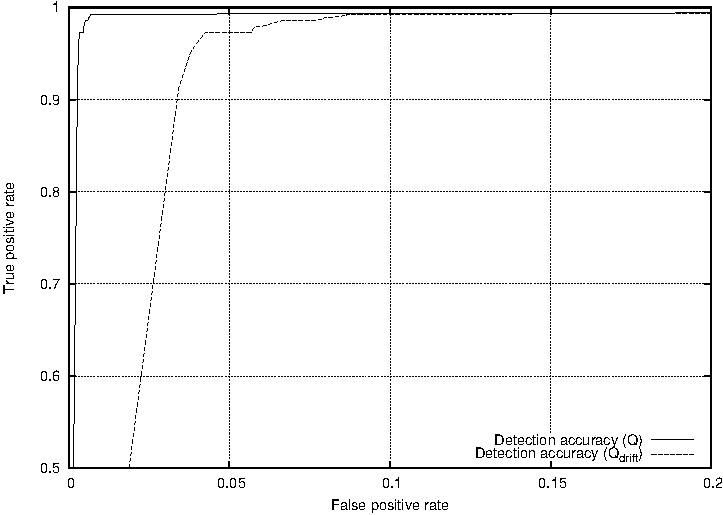
\includegraphics[width=0.48\textwidth]{figures/web/conceptdrift/fig_alerts}
    \label{fig:changes-increase-fpr}}
  \subfloat[Response modeling enabled.]{
    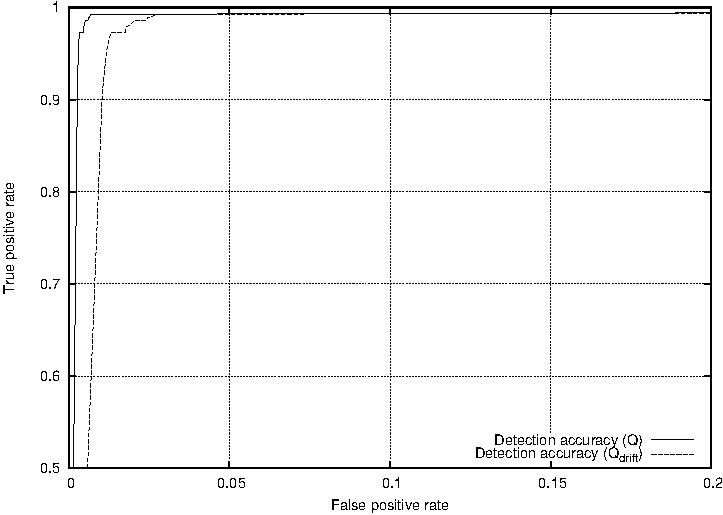
\includegraphics[width=0.48\textwidth]{figures/web/conceptdrift/fig_alerts_resp}
    \label{fig:response-models-fpr}}

  \caption{Detection and false positive rates measured on $Q$ and $Q_{\text{drift}}$, with \ac{HTTP}\index{HTTP} response modeling enabled in (b).}
\end{figure}

\subsubsection{Change detection}
\label{web:conceptdrift:eval:detection}
The second experiment quantifies the improvement in the detection accuracy of \webanomaly in the presence of web application change.  As before, the detector was trained over an unmodified filtered data set, and the resulting profiles were evaluated over both $Q$ and $Q_{\text{drift}}$.  In this experiment, however, the \ac{HTTP}\index{HTTP} response modeling technique was enabled.

Figure~\ref{fig:response-models-fpr} presents the results of analyzing \ac{HTTP}\index{HTTP} responses on detection accuracy.  Since many changes in the behavior of the web application and its clients can be discovered using our response modeling technique, the false positive rate for $Q_{\text{drift}}$ is greatly reduced over that shown in Figure~\ref{fig:changes-increase-fpr}, and approaches that of $Q$, where no changes have been introduced.  The small observed increase in false positive rate can be attributed to the effects of changes in parameter values.  This occurs because a change has been introduced into a parameter value submitted by a client to the web application, and no indication of this change was detected on the preceding document returned to the client (e.g., because no \texttt{<select />} were found).

Table~\ref{fig:fpr-table} displays the individual contributions to the reduction of the false positive rate due to the response modeling technique.  Specifically, the total number of anomalies caused by each type of change, the number of anomalies erroneously reported as alerts, and the corresponding reduction in the false positive rate is shown.  The results displayed were generated from a run using the optimal operating point (0.00144, 0.97263) indicated by the knee of the \ac{ROC}\index{ROC} curve in Figure~\ref{fig:response-models-fpr}.  For changes in session flows and parameters sets, the detector was able to identify an anomaly as being caused by a change in web application behavior in all cases.  This resulted in a large net decrease in the false positive rate of the detector with response modeling enabled.  The modification of parameters is more problematic, though; as discussed in Section~\ref{web:conceptdrift:design:discussion}, it is not always apparent that a change has occurred when that change is limited to the type of behavior a parameter's value exhibits.

\begin{table}[t]
  \centering
  \begin{tabular}{rccc}
    \toprule
    \textsc{Change type} & \textsc{Anomalies} & \textsc{FP} & \textsc{Reduction} \\
    \midrule
    New session flows & 6,749 & 0 & 100.0\% \\
    New parameters & 6,750 & 0 & 100.0\% \\
    Modified parameters & 5,785 & 4,821 & 16.6\% \\
    \cmidrule{2-4}
    \emph{Total} & 19,284 & 4,821 & 75.0\% \\
    \bottomrule
  \end{tabular}

  \caption{Reduction in the false positive rate due to \ac{HTTP}\index{HTTP} response modeling for various types of changes.}
  \label{fig:fpr-table}
  \vspace*{-.65cm}
\end{table}

From the overall improvement in false positive rates, we conclude that \ac{HTTP}\index{HTTP} response modeling is an effective technique for distinguishing between anomalies due to legitimate changes in web applications and those caused by malicious behavior.  Furthermore, any anomaly detector that does not do so is prone to generating a large number of false positives when changes do occur in the modeled application.  Finally, as it has been shown in Section~\ref{web:conceptdrift:motivation}, web applications exhibit significant long-term change in practice, and, therefore, concept drift is a critical aspect of web application anomaly detection that must be addressed.

\section{Concluding Remarks}
\label{web:conclusions}
In this chapter we described in detail two approaches to mitigate training issues. In particular, we presented a technique to reduce \acp{FP}\index{FP} due to scarce training data and a mechanism to automatically recognize changes in the monitored applications, such as code updates, and re-train the models without any human intervention.

First, we have described our efforts to cope with an issue that must be addressed by web application anomaly detection systems in order to provide a reasonable level of security.  The impact of this issue is particularly relevant for commercial web-based anomaly detection systems and web application firewall, which have to operate in real-world environment where sufficient training data might be unavailable within a reasonable time frame.

We have proposed the use of global knowledge bases of well-trained, stable profiles to remediate a local scarcity of training data by exploiting global similarities in web application parameters. We found that although using global profiles does result in a small reduction in detection accuracy, the resulting system, when given appropriate parameters, does provide reasonably precise modeling of otherwise unprotected web application parameters.

A possible future extension of the described approach is to investigate the use of other types of models, particularly \ac{HTTP}\index{HTTP} response and session models. An additional line of future work is the application of different clustering methods in order to improve the efficiency of the querying procedure for high-cardinality knowledge bases.

Secondly, we have identified the natural dynamicity of web applications as an issue that must be addressed by modern anomaly-based web application anomaly detectors in order to prevent increases in the false positive rate whenever the monitored web application is changed. We named this frequent phenomenon the \emph{web application concept drift}.

In \citep{2009_maggi_robertson_kruegel_vigna} we proposed the use of novel \ac{HTTP}\index{HTTP} response modeling techniques to discriminate between legitimate changes and anomalous behaviors in web applications. More precisely, responses are analyzed to find new and previously unmodeled parameters. This information is extracted from anchors and forms elements, and then leveraged to update request and session models. We have evaluated the effectiveness of our approach over an extensive real-world data set of web application traffic. The results show that the resulting system can detect anomalies and avoid false alerts in the presence of concept drift.

We plan to investigate the potential benefits of modeling the behavior of JavaScript\index{JavaScript} code, which is becoming increasingly prevalent in modern web applications. Also, additional, richer, and media-dependent response models must be studied to account for interactive client-side components, such as Adobe Flash and Microsoft Silverlight\index{Silverlight} applications.

%%% Local Variables: 
%%% mode: latex
%%% TeX-master: "thesis"
%%% End: 
